\documentclass[letterpaper]{article}
\usepackage[margin=1in]{geometry}

\usepackage{float}
\usepackage{amsmath}
\usepackage{amssymb}
\usepackage{multicol}
\usepackage{listings}
\usepackage{tikz}
\usepackage{gensymb}
\usepackage[hidelinks]{hyperref}
\usetikzlibrary{calc, shapes, arrows}
\usetikzlibrary{automata,positioning} % For NFA

\tikzstyle{decision} = [diamond, draw, text centered, minimum height=2em]
\tikzstyle{process} = [rectangle, draw, text centered, minimum height=2em]
\tikzstyle{terminator} = [rectangle, draw, text centered, rounded corners, minimum height=2em]
\tikzstyle{data}=[trapezium, draw, text centered, trapezium left angle=60, trapezium right angle=120, minimum height=2em]
\tikzstyle{connector} = [draw, -latex']
\tikzstyle{curve} = [draw]

\tikzstyle{block} = [draw, rectangle, 
    minimum height=3em, minimum width=3em]
\tikzstyle{sum} = [draw, circle, node distance=1cm]

\usepackage{enumitem}
\usepackage{tcolorbox}

\renewcommand\thesection{\Alph{section}.}
\renewcommand\thesubsection{\arabic{subsection}.}
\renewcommand\thesubsubsection{\Roman{subsubsection}.}

% Remove Indentation
\usepackage{parskip}

\begin{document}

\begin{titlepage}
    \vspace*{\stretch{2.0}}
    \begin{center}
       \Large\textbf{Adaptable House: Anti-Sway} \\
       \Large\textbf{Official Control/Software Manual and Documentation} \\
       \vspace*{\stretch{10.0}}
       \large{Espinola, Malachi P} \\
       \large{Hokenstad, Ethan T} \\
       \large{Neff, Callen P} \\
       \large{Nguyen, Tri V} \\
       \large{Tevy, Vattanary} \\
       \vspace*{\stretch{1.0}}
       \Large{University of Washington} \\
       \Large{Department of Mechanical Engineering} \\
    \end{center}
\end{titlepage}

\newpage

\tableofcontents

\newpage

\section{Introduction}
\subsection{Project Motive}
The Adaptable House Capstone, begun by Mary Meyer, envisions an ``adaptable house" capable of helping patients with neuralmuscular disease, disorders, and injuries. The goal is for this house to assist people to walk around with a system that supports them, and adapts to their movements. The Anti-Sway division of this capstone was in charge of proving that lateral movement support could be provided to such users. Thus, at the Univeristy of Washington, the Anti-Sway Capstone group developed, tested and verified a small scale system that could prove that it can be done. 
\subsection{Manual Coverage}
A small and yet significant portion of this system is the embedded software that forms the cornerstone of the system by providing robust control for patients using the system. This document will thus provide a guide through, and for:
\begin{enumerate}
    \item Software Design of Existing System
    \item Implementation Decisions at Project Time
    \item Future Integration for Lift Control
\end{enumerate}
\subsection{Manual Limitations}
Although this manual aims to serve as a generous guide through the system, it should be noted that the subjects discussed are beyond trivial, and as such, one should be familiar with both control theory and common software development trends (the latter of which changes rapidly), although this manual will attempt to provide some background.

In particular, it is not a reiteration of every single software function ever defined. Such scrutinizing details are well documented within the code. This manual is here chiefly to explain any complicated algorithms, and the high level concepts captured by the software.

\newpage

\section{Requirements}
\subsection{Client-Side Requirements}
Client-Side Requirements are simple:
\begin{enumerate}
    \item The user is safe at all times when using the support system
    \item The system provides varying levels of support during lateral movement
\end{enumerate}
\subsection{Interpreted Requirements}
Since we handle lateral movement, these are interpreted to measurement
\begin{enumerate}
    \item The user can walk around with varying levels of weight support
    \item The user can direct the system to move them with full-weight support.
    \item The system does not discomfort the user while doing so.
\end{enumerate}

% \newpage

% \section{Background}
% \subsection{A Brief Overview of Feedback Control}
% \subsection{Finite State Machines}
% \subsection{Software Design: Modularity}
% \subsection{Parallelism and Mutual Exclusion}
% \subsection{Microcomputers and C Programs}
% \subsubsection{Error Codes}
% \subsubsection{Memory Constraints}

\newpage

\section{Anti-Sway Control Modes and Schemes}
\subsection{Innate System (Plant)}
The system as set up essentially looks like the following:
\begin{figure}[H]
    \centering
    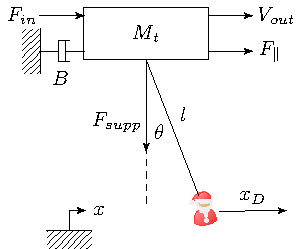
\includegraphics[width=10cm]{tracking_plant_diag_2.pdf}
    \begin{tabular}{@{}ll@{}}
        $F_{in}$ - \text{Applied Force} & $V_{out}$ - \text{Trolley Velocity} \\
        $F_{supp}$ - \text{Support Force} & $F_{\parallel}$ - \text{Parallel Support Force} \\
        $B$ - \text{Trolley Damping} & $M_{t}$ - \text{Trolley Mass} \\
        $\Theta$ - \text{Swing Angle} & $l$ - \text{String Length} \\
        $x_{D}$ - \text{Disturbance Motion} & \\
    \end{tabular}
    \caption{Plant Model}
    \label{plant}
\end{figure}
We have a few things to point out:
\begin{itemize}
    \item The mass $M_t$ represents the trolley that moves on the ceiling of the house.
    \item $l$ is the rope (which ends up being a rod within the desktop model) that connects the trolley to the user
\end{itemize}

In this case, the point of control is $F_{in}$, as that is the only thing the software can alter about the system.

\begin{tcolorbox}[colframe=red!75!black,colback=yellow!5, title=WARNING]
    In this case, all positive conventions are shown. In particular, the angle, force, and velocity are all positive in the direction of the positive lateral axis. These conventions must be obeyed in the software.
\end{tcolorbox}

Equivalently, the innate system, or the plant, can be represented using the following block diagram:
\begin{figure}[H]
    \centering
    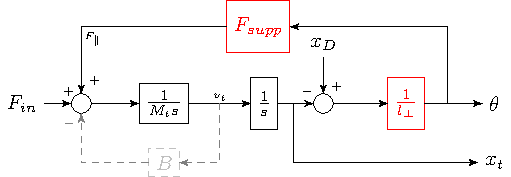
\includegraphics[width=10cm]{tracking_modified_plant_block.pdf}
\end{figure}

where the damping is or is not present in the system (due to either physical or control factors).

\subsection{Tracking Mode}
Tracking Mode is the first proposed mode of operation for this system. This mode allows the user to walk around a room with varying levels of weight support, as if the system were not there. For tracking mode, the strategy of control is shown below:
\begin{figure}[H]
    \centering
    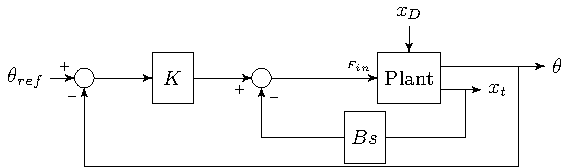
\includegraphics[width=10cm]{tracking_controller.pdf}
\end{figure}

Here, an outer-loop inner-loop sheme is used here.
\begin{itemize}
    \item In the outer loop, controller attempts to minimize the angle as much as possible while the user moves on the ground. The result is thus a tracking effect. 
    \item The inner-loop however, smoothens out the raw form of the outer-loop control, which helps result in a frictionless feel to this particular mode. In some respect, it can be viewed as velocity control, or the loop's attempt to control the velocity of the trolley. However, it is moreso an impedence controller as it introduces artificial damping into the system. This is consistent with the smoothing effect just mentioned.
\end{itemize}

\subsection{Anti-Sway Mode}

The second proposed mode is Anti-Sway Mode. This mode is meant to be used when the person is suspended in the system. In this mode, the person can direct the system using a remote control, while the mode does not allow the person to sway. The scheme for anti-sway mode is shown below:

\begin{figure}[H]
    \centering
    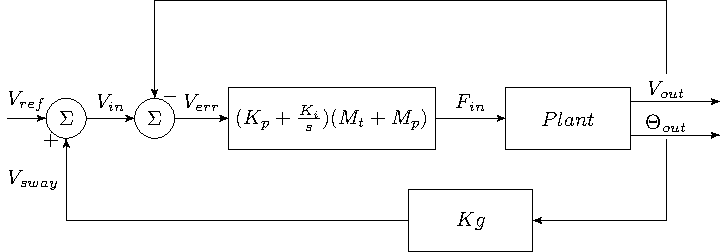
\includegraphics[width=10cm]{antisway_block.pdf}
\end{figure}

Essentially, the main purpose of this scheme is to prevent the user from swaying during movement. This is also a form of inner-loop outer-loop control, but the purposes of each are different:
\begin{itemize}
    \item The outer-loop takes the reference velocity, as specified by the user via a remote control (in our case, the LCD keypad), and modulates by adding a proportion of the angle. This is the anti-sway portion of the control. Initially, as the angle of the rope deviates from the reference, the velocity is moduled to dampen out any sway that can result. Then, as the angle returns to reference, the person is allowed to move to their reference velocity.
    \item The inner-loop is a velocity control, which helps the user optimally follow the velocity planned by the outer-loop. It uses a PI controller with a specific form optimized to the masses of the system.
\end{itemize}

\subsection{Force to Voltage Conversion}
Both control schemes shown output a force to the plant, but in the physical system, one should notice that is impossible, because we use motors to output this force, but we can only do so via outputting a voltage to the motor, which then allows the motor to convert it to a force. Thus to achieve the $F_{in}$ is applied to the plant in both control schemes, the following voltage is sent out:
$$\boxed{V_{in}=\frac{r}{K_aK_m}F_{in}}$$
where $r$ is the radius of the pulley connected to the motor shaft, $K_a$ is the Amplifier Constant, and $K_m$ is the motor constant (more information in the Final Capstone Paper).

\newpage
\section{Hardware Specifications}
When going into the Hardware Specifications, please note that this is not at all an in depth analysis into these systems. More information can be found in the corresponding final paper for this Capstone.
\subsection{Microcomputer}
The microcomputer being used is the National Instruments MyRIO, an embedded computer that was used mainly since it was the choice embedded system used by students in the Mechatronics Capstone of the University of Washington. More information about this microcomputer can be found here: \hyperlink{https://www.ni.com/en/shop/engineering-education/portable-student-devices/myrio-student-embedded-device/what-is-myrio.html}{MyRio Information}.
\subsection{Mechanical Frame}
The portion of the mechanical frame that was used to contain the trolley and allow it to move around is a modified Laser Engraver, which can be found here \hyperlink{https://www.vevor.com/laser-engraving-machine-c_11141/vevor-laser-engraver-laser-engraving-machine-5w-compressed-spot-eye-protection-p_010907755157}{Vevor Laser Engraver}. In particular the following attributes were modified:
\begin{itemize}
    \item Laser: Replaced with trolley
    \item Motors: Replaced with DC motors (required 3D printed adapters to fit)
\end{itemize}
To raise this portion up, aluminum maker beams where used to make a simple lower frame, whose purpose is to simply raise the modified laser engraver.
Finally, to model a harness attachement to the user, a metal rod attached to a ball (to represent the user) and the trolley was used.

\section{Sensor/Actuator Specifications}
For this section, this is not an extensive overview of the hardware. For that, please refer to the Capstone Final Paper.
\subsection{Angle Sensing: Potentiometers}
To sense the angle of the harness, which is the metal rod in this case, 2 rotary potentiometers were used. Since its output voltage changes linearly (approximately) with the amount of rotation its rotor has undergone, it was a simple way to obtain the angle of the rod. Of course, in order for them to mirror the angle of the rod, part of the trolley is designed to help attach the potentiometers to the rod to do so (more information can be found in the Capstone Paper).
\subsubsection{Calibration Method and Results}
To calibrate the potentiometers (that is, to come up with the ratio of voltage change in the potentiometer output to the change in the rod angle), measurements of the potentiometer voltage with rod being at 3 different angles were performed for both potentiometers. Assuming a linear relationship, one simply can apply the formula:
$$m=\frac{\theta_2-\theta_1}{V_1-V_2}$$
with this formula, 2 slopes were obtained, and the average of the two resulted in the value of:
$$\boxed{m=2.11 \frac{\degree}{V} = 0.0368 \frac{rad}{V}}$$
which the embedded code uses to interpret the potentiometer voltage into a rod angle.
\subsection{Position Sensing: Encoders}
For this application, the encoders used were HEDS 5540 A11 quadrature encoders.
\subsection{Force Actuation: Motor}
For this application, custom Swiss Maxon motors where used.
\subsection{Velocity Actuation: Keypad}
In a way, the remote control held by the person during anti-sway. This is emulated by the use of the LCD keypad that comes with the MyRio. Of course, additional programming must be done to support this, which is discussed later.

\newpage

\section{Embedded Software} \label{section-emb-soft}
The following sections exclude discussion of \texttt{main.c}, which technically runs the program via its use of a main method. However, it is realtively simplistic, and simply calls on the system to start. The following sections will then discuss it.

\subsection{System Setup/Shutdown: \texttt{setup}}
This module is probably the simplest in concept. It is in charge of calling all modules' global startup and shutdown functions, which are one time only functions. The modules that depend on this are the MyRIO FPGA (\texttt{MyRio.h}), the Sensor/Actuator Module (\texttt{io.h}), and the data recording module (\texttt{record.h}), as shown in Figure \ref{setup-mdd}:
\begin{figure}[h]
    \centering
    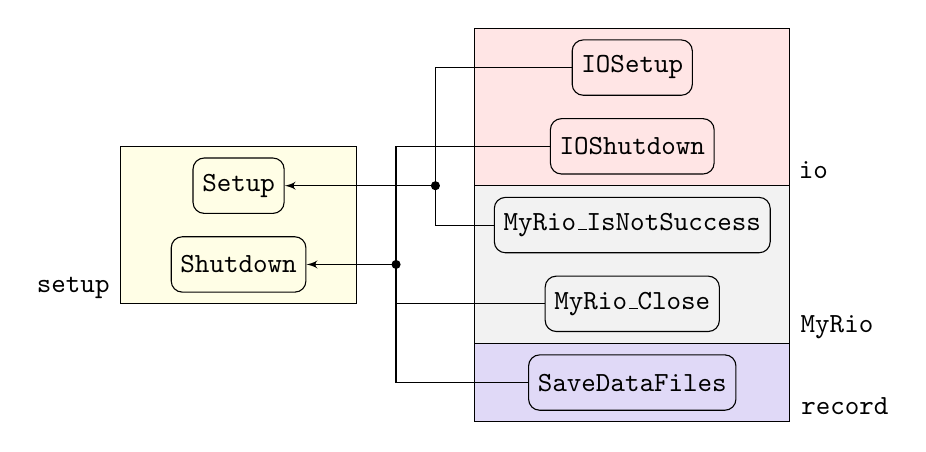
\begin{tikzpicture}
        
        \node[rectangle, draw, minimum width=3cm, minimum height=2cm, fill=yellow!10] (setup) at (-3, -1) {};
        \node at (-5.1, -1.8) {\texttt{setup}}; 
        \node[terminator] at (-3, -0.5) (Setup) {\texttt{Setup}};
        \node[terminator] at (-3, -1.5) (Shutdown) {\texttt{Shutdown}};
        
        \node[rectangle, draw, minimum width=4cm, minimum height=2cm, fill=red!10] (io) at (2, 0.5) {};
        \node at (4.3, -0.3) {\texttt{io}};
        \node[terminator] at (2, 1) (IOSetup) {\texttt{IOSetup}};
        \node[terminator] at (2, 0) (IOShutdown) {\texttt{IOShutdown}};
        
        \node[rectangle, draw, minimum width=4cm, minimum height=2cm, fill=gray!10] (MyRio) at (2, -1.5) {};
        \node at (4.6, -2.3) {\texttt{MyRio}};
        \node[terminator] at (2, -1) (MyRio_IsNotSuccess) {\texttt{MyRio\_IsNotSuccess}};
        \node[terminator] at (2, -2) (MyRio_Close) {\texttt{MyRio\_Close}};
        
        \node[rectangle, draw, minimum width=4cm, minimum height=1cm, fill=blue!80!red!15] (record) at (2, -3) {};
        \node at (4.7, -3.3) {\texttt{record}};
        \node[terminator] at (2, -3) (SaveDataFiles) {\texttt{SaveDataFiles}};

        \draw[connector] (IOSetup) -- (-0.5, 1) -- (-0.5, -0.5) -- (Setup);
        \draw[connector] (IOShutdown) -- (-1, 0) -- (-1, -1.5) -- (Shutdown);

        \draw[-] (MyRio_IsNotSuccess) -- (-0.5, -1) -- (-0.5, -0.5);
        \draw[-] (MyRio_Close) -- (-1, -2) -- (-1, -1.5);

        \draw[-] (SaveDataFiles) -- (-1, -3) -- (-1, -2);

        \filldraw[color=black] (-0.5, -0.5) circle (0.05);
        \filldraw[color=black] (-1, -1.5) circle (0.05);
        
    \end{tikzpicture}
    \caption{\texttt{setup} Module Dependency Diagram}
    \label{setup-mdd}
\end{figure}

It has two methods (both of which are \texttt{extern}):
\begin{enumerate}
    \item \texttt{int Setup()}: Starts the System
    \item \texttt{int Shutdown()}: Stops the System
\end{enumerate}
which both call the setup and shutdown functionality of the dependent modules, and return the conventional error code to signal if any of the dependent modules fail to initialize/deallocate. In particular, both methods start and stop:
\begin{enumerate}
    \item The ability to utilize the MyRio's FPGA (via \texttt{MyRio})
    \item The ability to interface with Sensors/Actuators (via \texttt{io})
    \item (For \texttt{Shutdown()} only) Writing all Data to MyRio's Disk (via \texttt{Record})
\end{enumerate}

It is also responsible for initializing the universal error code, which will be discussed later, but is an error signal shared accross threads with specific codes (somewhat related to the C construct of \texttt{errno}).

\subsubsection{Calibration: Setting up \texttt{io}}
Although it is strange to talk about another module within this context, talking about system initialization through \texttt{io} is appropriate here. The \texttt{io} module has to know what the reference position and angle are. To do so, it requests that the user set the trolley and the angle to the desired reference, and then sets it, all during the \texttt{IOSetup()} method. For reference, the displayed prompt is:

\begin{center}
    \begin{lstlisting}
        Please stablize for calibration.
        Press ENTR when ready._
    \end{lstlisting}
\end{center}

More information about this particular method can be found in Section \ref{section-emb-soft}\ref{subsection-io} which will go into the specifics as to how exactly that is done.

\newpage

\subsection{System Management: \texttt{system}}
The \texttt{system} module is essentially responsible for running the entire software. It obviously does so by deffering basically each ``action'' to the other modules, so just like the \texttt{io} module, it does not really do a lot of heavy lifting. However, as the abstract representation of the system itself, it should be no surprise that its design resembles a Turing Machine (or a View/Controller, if you are familiar with the Model-View-Controller Software Design Pattern). Its interface is a simple function:
\begin{itemize}
    \item \texttt{int SystemExec()\footnote{Notice the \texttt{Exec} attached to the end of the name, which references the illusion that it is its own program and returns a conventional status code. This function does not actually clone the embedded process, its just a fun naming convention.}}: Executes the System
\end{itemize}
Now, we shall discuss how the system is structured on a high level. The following Finite State Automata, defined as a Nondeterministic Finite Automata (NFA)\footnote{This particular version of a Turing Machine is being invoked for simplicity, but also because the input to the \texttt{system} is quite literally a senary (base-6) string}, shows the state transitions for the System. Let us define the alphabet to be:
$$\boxed{A := \left\{1, 2, 3, 4, \leftarrow, E\right\}}$$
where $1-4$ are keypad keys, $\leftarrow$ is the keypad delete key, and $E$ is a universal error (with $\epsilon$ as the empty string/character). Then:
\begin{figure}[H]
    \centering
    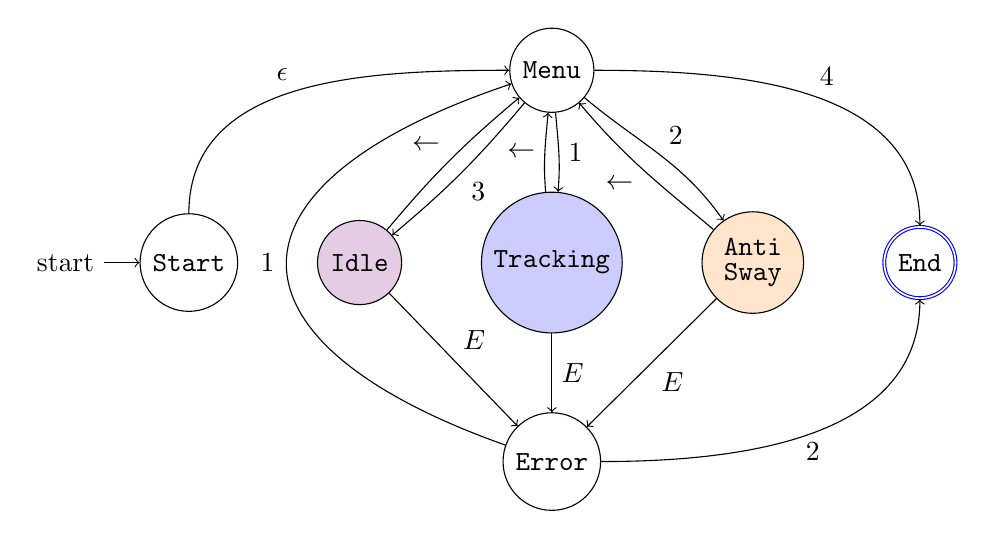
\begin{tikzpicture}
        \node[state, initial] (Start) {\texttt{Start}};
        \node[state, right =of Start, fill=violet!20] (Idle) {\texttt{Idle}};
        \node[state, right=of Idle, fill=blue!20] (Tracking) {\texttt{Tracking}};
        \node[state, right=of Tracking, fill=orange!20] (Anti-Sway) {\shortstack{\texttt{Anti}\\\texttt{Sway}}};
        \node[state, above =of Tracking] (Menu) {\texttt{Menu}};
        \node[state, below=of Tracking] (Error) {\texttt{Error}};
        \node[state, accepting, right= of Anti-Sway, draw=blue!100!black!100] (End) {\texttt{End}};

        \path[->]
        (Start) edge [out=90, in=180] node [above left] {$\epsilon$} (Menu)
        (Menu) edge [out=-130, in=40] node [below right] {$3$} (Idle)
               edge [out=-85, in=85] node [right] {$1$} (Tracking)
               edge [out=-40, in=125] node [above right] {$2$} (Anti-Sway)
        (Anti-Sway) edge [out=140, in=-50] node [below left] {$\leftarrow$} (Menu)
                    edge node [below right] {$E$} (Error)
        (Tracking) edge [out=95, in=-95] node [left] {$\leftarrow$} (Menu)
                   edge node [right] {$E$} (Error)
        (Idle) edge [out=50, in=-140] node [above left] {$\leftarrow$} (Menu)
               edge node [above right] {$E$} (Error)
        (Error) edge [out=0, in=270] node [below] {$2$} (End)
        (Menu) edge [out=0, in=90] node [above right] {$4$} (End);

        \node at (1, 0) {$1$};
        \draw[->] (Error) .. controls (0.3, -1) and (0.3, 1).. (Menu);
    \end{tikzpicture}
    \label{system-nfa}
    \caption{NFA for \texttt{system}}
\end{figure}
Note the correspondence of the 2 anti-sway modes with both the Tracking and Anti-Sway States. The presence of an idle mode is merely to check that sensors are working properly, it is not an actual control mode.

Implementing \texttt{system} becomes very straightforward from inspecting Figure \ref{system-nfa}. A function is assigned to each state, which are each responsible for indicating the next state to execute as well as executing the appropriate actions for that state, while all \texttt{SystemExec()} does is manage these states' execution flow. The dependency diagram for the \texttt{system} module is now shown in Figure \ref{system-mdd} (next page).
\begin{figure}[H]
    \centering
    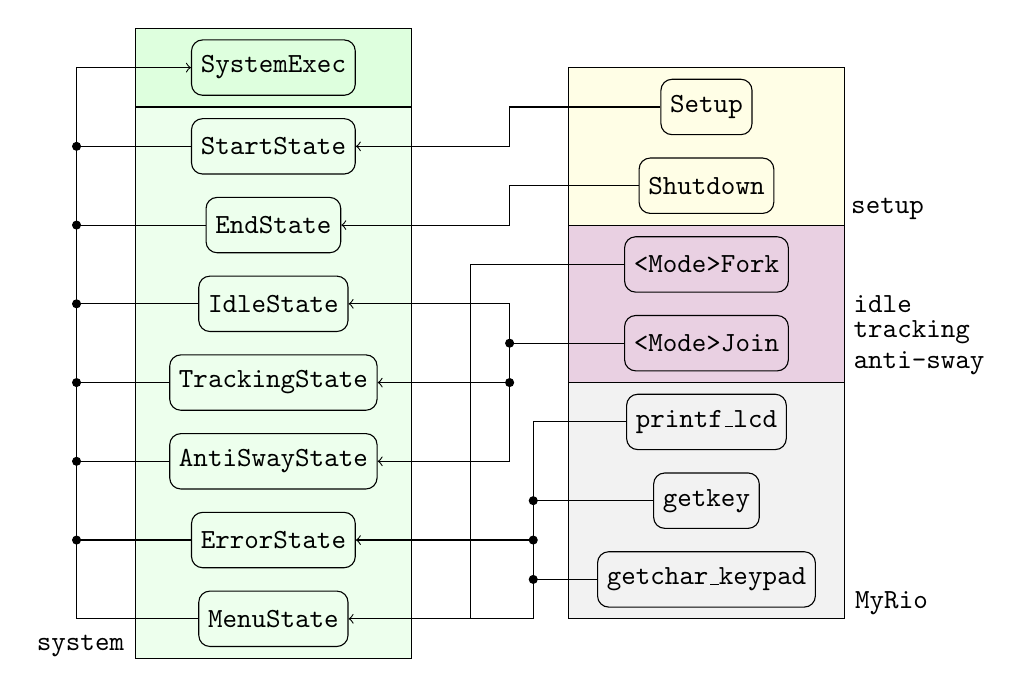
\begin{tikzpicture}

        \node[rectangle, draw, minimum width=3.5cm, minimum height=1cm, fill=green!13] at (0, 0) {};
        \node[rectangle, draw, minimum width=3.5cm, minimum height=7cm, fill=green!7] at (0, -4) {};
        \node at (-2.45, -7.35) {\texttt{system}};
        \node[terminator] at (0, 0) (SystemExec) {\texttt{SystemExec}};
        \node[terminator] at (0, -1) (StartState) {\texttt{StartState}};
        \node[terminator] at (0, -2) (EndState) {\texttt{EndState}};
        \node[terminator] at (0, -3) (IdleState) {\texttt{IdleState}};
        \node[terminator] at (0, -4) (TrackingState) {\texttt{TrackingState}};
        \node[terminator] at (0, -5) (Anti-SwayState) {\texttt{AntiSwayState}};
        \node[terminator] at (0, -6) (ErrorState) {\texttt{ErrorState}};
        \node[terminator] at (0, -7) (MenuState) {\texttt{MenuState}};

        \node[rectangle, draw, minimum width=3.5cm, minimum height=2cm, fill=yellow!10] at (5.5, -1) {};
        \node at (7.8, -1.8) {\texttt{setup}};
        \node[terminator] at (5.5, -0.5) (Setup) {\texttt{Setup}};
        \node[terminator] at (5.5, -1.5) (Shutdown) {\texttt{Shutdown}};

        \node[rectangle, draw, minimum width=3.5cm, minimum height=2cm, fill=blue!20!orange!20!violet!20] at (5.5, -3) {};
        \node at (8.2, -3.4) {\texttt{\shortstack[l]{\texttt{idle}\\\texttt{tracking}\\\texttt{anti-sway}}}};
        \node[terminator] at (5.5, -2.5) (ModeFork) {\texttt{<Mode>Fork}};
        \node[terminator] at (5.5, -3.5) (ModeJoin) {\texttt{<Mode>Join}};

        \node[rectangle, draw, minimum width=3.5cm, minimum height=3cm, fill=gray!10] at (5.5, -5.5) {};
        \node at (7.85, -6.8) {\texttt{MyRio}};
        \node[terminator] at (5.5, -4.5) (printf_lcd) {\texttt{printf\_lcd}};
        \node[terminator] at (5.5, -5.5) (getkey) {\texttt{getkey}};
        \node[terminator] at (5.5, -6.5) (getchar_keypad) {\texttt{getchar\_keypad}};

        \draw[->] (Setup) -- (3, -0.5) -- (3, -1) -- (StartState);
        \draw[->] (Shutdown) -- (3, -1.5) -- (3, -2) -- (EndState);
        \draw[->] (ModeFork) -- (2.5, -2.5) -- (2.5, -7) -- (MenuState);
        \draw[->] (ModeJoin) -- (3, -3.5) -- (3, -3) -- (IdleState);
        \draw[->] (3, -3.5) -- (3, -4) -- (TrackingState);
        \draw[->] (3, -4) -- (3, -5) -- (Anti-SwayState);
        \draw[->] (printf_lcd) -- (3.3, -4.5) -- (3.3, -6) -- (ErrorState);
        \draw[-] (3.3, -6) -- (3.3, -7) -- (2.5, -7);
        \draw[-] (getkey) -- (3.3, -5.5);
        \draw[-] (getchar_keypad) -- (3.3, -6.5);

        \draw[<-] (SystemExec) -- (-2.5, 0) -- (-2.5, -7) -- (MenuState);
        \draw[-] (-2.5, -1) -- (StartState);
        \draw[-] (-2.5, -2) -- (EndState);
        \draw[-] (-2.5, -3) -- (IdleState);
        \draw[-] (-2.5, -4) -- (TrackingState);
        \draw[-] (-2.5, -5) -- (Anti-SwayState);
        \draw[-] (-2.5, -6) -- (ErrorState);

        \filldraw[color=black] (3, -3.5) circle (0.05);
        \filldraw[color=black] (3, -4) circle (0.05);
        \filldraw[color=black] (3.3, -5.5) circle (0.05);
        \filldraw[color=black] (3.3, -6) circle (0.05);
        \filldraw[color=black] (3.3, -6.5) circle (0.05);

        \filldraw[color=black] (-2.5, -1) circle (0.05);
        \filldraw[color=black] (-2.5, -2) circle (0.05);
        \filldraw[color=black] (-2.5, -3) circle (0.05);
        \filldraw[color=black] (-2.5, -4) circle (0.05);
        \filldraw[color=black] (-2.5, -5) circle (0.05);
        \filldraw[color=black] (-2.5, -6) circle (0.05);

    \end{tikzpicture}
    \caption{\texttt{system} Module Dependency Diagram}
    \label{system-mdd}
\end{figure}

The description of such functions follows:
\begin{itemize}
    \item \texttt{static int StartState()}: Dedicated to setting up the System (by setting it up via \texttt{Setup()})
    \item \texttt{static int EndState()}: Dedicated to stopping the System (by shutting it down \texttt{Shutdown()})
    \item \texttt{static int IdleState(), TrackingState(), AntiSwayState()}: Runs the corresponding state, and exits them when $\leftarrow$ is pressed or a universal error occurs
    \item \texttt{static int ErrorState()}: Processes a universal error with user input
    \item \texttt{static int MenuState()}: Allows the user to choose any of the Modes, and navigates to it
\end{itemize}
To acomplish state execution and state transitions, the following data types are employed:
\begin{multicols}{2}
    \begin{center}
        \begin{lstlisting}[language=C]
            enum {
                ANTI_SWAY,
                TRACKING,
                IDLE,
                MENU,
                ERROR,
                START,
                END
            } state = START;
                \end{lstlisting}
    \end{center}
    
    \columnbreak
    \begin{center}
        \begin{lstlisting}[language=C]
        static int (* states[])()
            = {AntiSwayState,
                TrackingState,
                IdleState,
                MenuState,
                ErrorState,
                StartState,
                EndState};
            \end{lstlisting}
    \end{center}
\end{multicols}
Thus, any State Function can set the variable \texttt{state} using the \texttt{enum} constants, and all \texttt{SystemExec()} needs to do to continue execution flow is state the line: \texttt{states[state]()}.

\begin{tcolorbox}[colframe=blue!50!black!70,title=Future Modification]
    Notice it is very critical for these fields to align in both the \texttt{enum} and the \texttt{states} array, and for all functions in the array to have the exact same function signature (save the name of course).
\end{tcolorbox}

\subsubsection{System Operation}
Upon startup, the following message will appear:
\begin{center}
    \begin{lstlisting}
        Please stablize for calibration.
        Press ENTR when ready._
    \end{lstlisting}
\end{center}
After moving the trolley to the desired reference position, and making it still, the user calibrates the system, and then we enter normal operation. Normal operation is marked by the MENU state, which displays the following prompt:
\begin{center}
    \begin{lstlisting}
        Indicate a mode:
        1) Tracking
        2) Anti-Sway
        3) Idle, 4) Exit
    \end{lstlisting}
\end{center}
After which the user enters a number, and then presses enter to start the corresponding mode (or exit)
While in a mode, the user can press the $\leftarrow$ key to exit the mode, but the mode will stay in operation until that is done, or, until the error state is triggered. If the error is recoverable, a prompt like the one below will show:
\begin{lstlisting}
        Error: An encoder(s) has failed..
        Press:
        1) Continue
        2) Exit
\end{lstlisting}
after which the user simply has to press 1 to reenter the menu state, or 2 to exit the program.
\newpage

\subsection{Thread Management: \texttt{thread-lib}}

The C Threading Library, \texttt{pthread}, is somewhat difficult to actually use. It can be confusing at times, and combined with the steps before we can start a thread within the MyRio embedded system, things get complicated really fast. That's why we make use of a library dedicated to making the process of threading easier. However, it does not define functions, instead it defines macros. Our dependency diagram is thus made up of macros:

\begin{figure}[H]
    \centering
    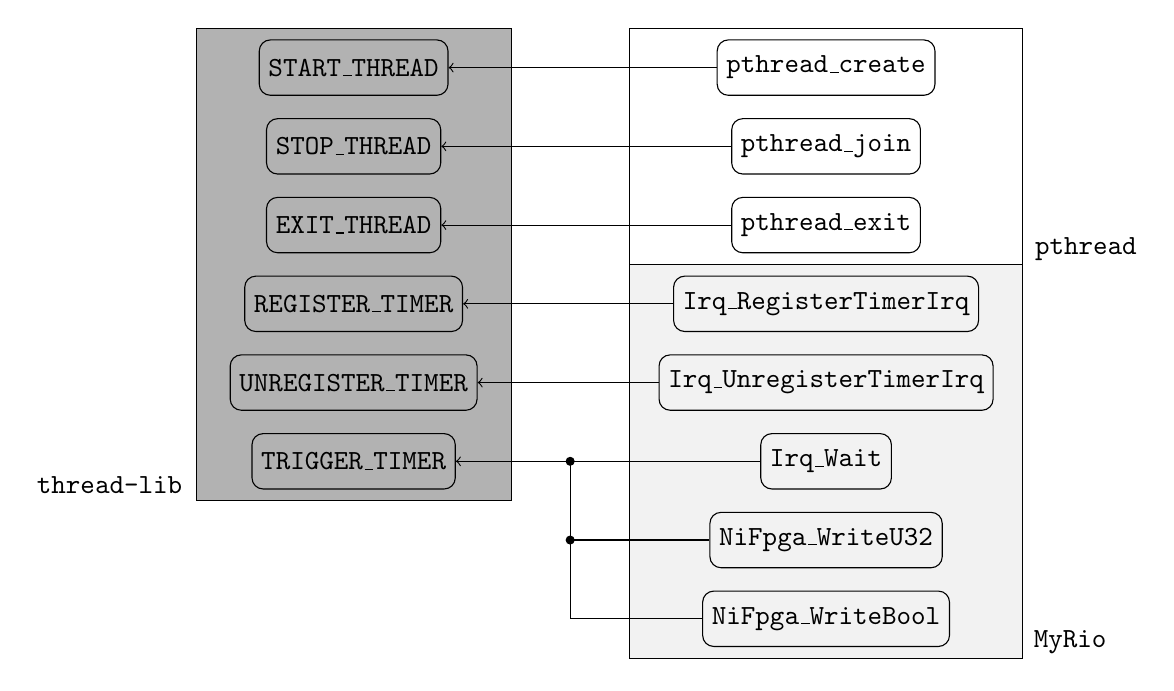
\begin{tikzpicture}
        \node[rectangle, draw, minimum width=4cm, minimum height=6cm, fill=black!30] at (0, -2.5) {};
        \node at (-3.1, -5.3) {\texttt{thread-lib}};
        \node[terminator] at (0, 0) (START_THREAD) {\texttt{START\_THREAD}};
        \node[terminator] at (0, -1) (STOP_THREAD) {\texttt{STOP\_THREAD}};
        \node[terminator] at (0, -2) (EXIT_THREAD) {\texttt{EXIT\_THREAD}};
        \node[terminator] at (0, -3) (REGISTER_TIMER) {\texttt{REGISTER\_TIMER}};
        \node[terminator] at (0, -4) (UNREGISTER_TIMER) {\texttt{UNREGISTER\_TIMER}};
        \node[terminator] at (0, -5) (TRIGGER_TIMER) {\texttt{TRIGGER\_TIMER}};

        \node[rectangle, draw, minimum width=5cm, minimum height=3cm] at (6, -1) {};
        \node at (9.3, -2.3) {\texttt{pthread}};
        \node[terminator] at (6, 0) (pthread_create) {\texttt{pthread\_create}};
        \node[terminator] at (6, -1) (pthread_join) {\texttt{pthread\_join}};
        \node[terminator] at (6, -2) (pthread_exit) {\texttt{pthread\_exit}};

        \node[rectangle, draw, minimum width=5cm, minimum height=5cm, fill=gray!10] at (6, -5) {};
        \node at (9.1, -7.3) {\texttt{MyRio}};
        \node[terminator] at (6, -3) (Irq_RegisterTimerIrq) {\texttt{Irq\_RegisterTimerIrq}};
        \node[terminator] at (6, -4) (Irq_UnregisterTimerIrq) {\texttt{Irq\_UnregisterTimerIrq}};
        \node[terminator] at (6, -5) (Irq_Wait) {\texttt{Irq\_Wait}};
        \node[terminator] at (6, -6) (NiFpga_WriteU32) {\texttt{NiFpga\_WriteU32}};
        \node[terminator] at (6, -7) (NiFpga_WriteBool) {\texttt{NiFpga\_WriteBool}};

        \draw[->] (pthread_create) -- (START_THREAD);
        \draw[->] (pthread_join) -- (STOP_THREAD);
        \draw[->] (pthread_exit) -- (EXIT_THREAD);
        \draw[->] (Irq_RegisterTimerIrq) -- (REGISTER_TIMER);
        \draw[->] (Irq_UnregisterTimerIrq) -- (UNREGISTER_TIMER);
        \draw[->] (Irq_Wait) -- (TRIGGER_TIMER);
        \draw[-] (NiFpga_WriteU32) -| (2.75, -5);
        \draw[-] (NiFpga_WriteBool) -| (2.75, -6);

        \filldraw[color=black] (Irq_Wait)++(-6+2.75, 0) circle (0.05);
        \filldraw[color=black] (NiFpga_WriteU32)++(-6+2.75, 0) circle (0.05);
    \end{tikzpicture}
\end{figure}

Like the \texttt{io} module, these macros simply serve as wrappers for processes that are difficult to write out, and as such, almost all macros only have one dependent function. We will now explain the macros:
\begin{itemize}
    \item \texttt{START\_THREAD(thread, function, resource)}: Starts a thread using a function, and passing in resource to the function, returning a non-zero value upon error.
    \item \texttt{STOP\_THREAD(thread, resource)}: Stops a Thread via its resource from the parent thread, returning a non-zero value upon error.
    \item \texttt{EXIT\_THREAD()}: Forces a thread to kill itself (so within itself).
    \item \texttt{REGISTER\_TIMER(resource)}: Registers the global timer with a thread given this resource.
    \item \texttt{UNREGISTER\_TIMER(resource)}: Unregisters the global timer from a thread associated with this resource.
    \item \texttt{TIMER\_TRIGGER(irq\_assert, resource)}: Triggers a timer in its default setting, and resets the timer and runs it again.
\end{itemize}

As you can see these names are self explanatory. They are the main event of this module, and they support something we dub (or rather stole) as the Fork-Join Framework.

Another thing this module does is that it defines the \texttt{ThreadResource} data structure, which is a data type that is passed to all thread functions in this framework. It also defines several macros that are consistent to all threads, which are physical constants about the system, as well as the length of a timestep, which is referred to as a BTI (Base Time Increment).

\newpage

\subsubsection{Streamlined Multithreading: Fork-Join Framework}
The macros provided in this module support a style of parallelism called Fork-Join\footnote{This is an illusion to Java's Fork-Join Framework, but that is obviously not in use here}. Essentially, use of this library should be done by implementing 3 functions:

\begin{multicols}{2}
    \begin{lstlisting}[language=C]
int Fork() {
    REGISTER_TIMER(thread_resource);
    START_THREAD(thread,
                 ThreadFunction,
                 thread_resource);
    return EXIT_SUCCESS;
}
    \end{lstlisting}
    \columnbreak
    \begin{lstlisting}[language=C]
int Join() {
    STOP_THREAD(thread);
    UNREGISTER_TIMER(thread_resource);
    return EXIT_SUCCESS;
}
    \end{lstlisting}
    
\end{multicols}


\begin{center}
    \begin{lstlisting}[language=C]
void *ThreadFunction(void *resource) {
    ThreadResource *thread_resource =
        (ThreadResource *) resource;

    while (resource->irq_thread_rdy) {
        int32_t irq_assert;
        TRIGGER_TIMER(irq_assert,
                      resource);

        if (irq_assert) {
            ...
        }
    }

    EXIT_THREAD();
}
    \end{lstlisting}
\end{center}

The use of all the timer and \texttt{irq\_assert} stuff is optional if you don't want your thread's main content to execute every 5 ms, but otherwise, you would need it. This however, is the Fork-Join Framework that this module supports, and it makes parallelism easier to look at!

\newpage

\subsection{Sensor/Actuator Interfacing: \texttt{io}} \label{subsection-io}
This module is quite complex, although its intention is simple. It is a decorator module over Sensor/Actuator accessor/mutator functions. There are a few reasons for this:
\begin{itemize}
    \item Ability to convert raw outputs from sensor functions, which are usually in non-usable formats (wrong units).
    \item Ability to monitor raw inputs into actuator functions, which alone can result in system/physical malfunction.
    \item Decorator functions provide ease of access and readability to both kinds of devices by reducing the amount of lines written (code reuse).
\end{itemize}
For each sensors/actuators, a variable of some data type defined by the MyRio I/O interfaces must be employed. Through its lifetime, that data type must have some way to:
\begin{enumerate}
    \item Initialized (Once)
    \item Use
    \item Delete (Once)
\end{enumerate}
\begin{tcolorbox}[colback=yellow!10, colframe=green!20!black!70, title=C-Style Usage]
    This is a very common design pattern used in C libraries that offer an interface to some data type. More explicitly, the above three functions usually come in the form:
    \begin{lstlisting}
        // Allocate/Initialize var (of type varType) with some parameters
        int AllocVar(..., varType *var);
        
        // Use var with some parameters
        int UseVar(varType *var, ...);
        
        // Free/Delete var (usually without parameters)
        int FreeVar(varType *var);
    \end{lstlisting}
    It resembles object oriented programing with memory managment, but obviously since C isn't object-oriented, it must externally offer functions that do the above 3 on a pointer to the variable of concern. What's more is that this style allows the user to fully control the allocation of the variable. This is important because you'll see this \underline{everywhere}, including in our code.
\end{tcolorbox}
Since this is true for all the sensors/actuator we use, you'll find these functions that do such things being used in obvious places. 

Of the data structures used in this module, the most interesting ones will be custom defined structures that represent 2D Position, Velocity, and Angle (i.e. \texttt{Positions}, \texttt{Velocities}, \texttt{Angles}), as well as aliasing for their unit counterparts (i.e. \texttt{Position}, \texttt{Velocity}, \texttt{Angle}) and \texttt{Voltage}, which are of an aliased floating point type we name \texttt{decimal}, for control over their underlying types. This is simply for convenience, but as you will soon see, they help us efficiently and intuitively hold sensor/actuator parameters/results for us.

Below is the dependency diagram for the \texttt{io} module, which wraps this functionality:
\begin{figure}[H]
    \centering
    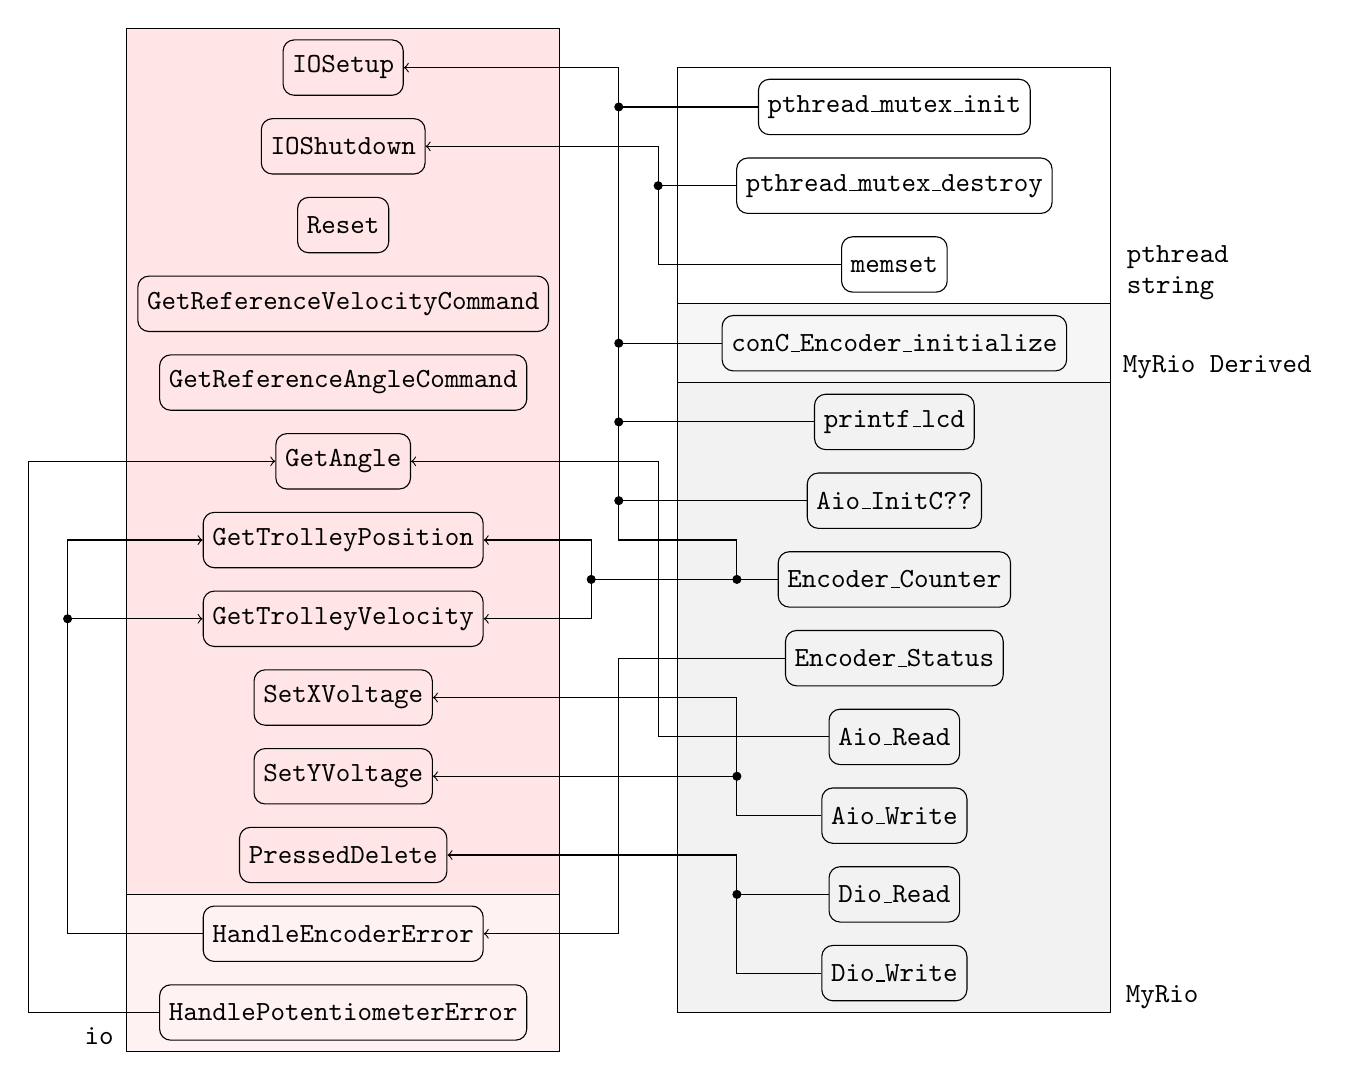
\begin{tikzpicture}
        \node[rectangle, draw, minimum width=5.5cm, minimum height=11cm, fill=red!10] at (0, -5) {};
        \node at (-3.1, -12.3) {\texttt{io}};
        \node[rectangle, draw, minimum width=5.5cm, minimum height=2cm, fill=red!5] at (0, -11.5) {};
        \node[terminator] at (0, 0) (IOSetup) {\texttt{IOSetup}};
        \node[terminator] at (0, -1) (IOShutdown) {\texttt{IOShutdown}};
        \node[terminator] at (0, -2) (Reset) {\texttt{Reset}};
        \node[terminator] at (0, -3) (GetReferenceVelocityCommand) {\texttt{GetReferenceVelocityCommand}};
        \node[terminator] at (0, -4) (GetReferenceAngleCommand) {\texttt{GetReferenceAngleCommand}};
        \node[terminator] at (0, -5) (GetAngle) {\texttt{GetAngle}};
        \node[terminator] at (0, -6) (GetTrolleyPosition) {\texttt{GetTrolleyPosition}};
        \node[terminator] at (0, -7) (GetTrolleyVelocity) {\texttt{GetTrolleyVelocity}};
        \node[terminator] at (0, -8) (SetXVoltage) {\texttt{SetXVoltage}};
        \node[terminator] at (0, -9) (SetYVoltage) {\texttt{SetYVoltage}};
        \node[terminator] at (0, -10) (PressedDelete) {\texttt{PressedDelete}};
        \node[terminator] at (0, -11) (HandleEncoderError) {\texttt{HandleEncoderError}};
        \node[terminator] at (0, -12) (HandlePotentiometerError) {\texttt{HandlePotentiometerError}};

        
        \node[rectangle, draw, minimum width=5.5cm, minimum height=3cm] at (7, -1.5) {};
        \node at (10.6, -2.6) {\texttt{\shortstack[l]{pthread\\string}}};
        \node[terminator] at (7, -0.5) (pthread_mutex_init) {\texttt{pthread\_mutex\_init}};
        \node[terminator] at (7, -1.5) (pthread_mutex_destroy) {\texttt{pthread\_mutex\_destroy}};
        \node[terminator] at (7, -2.5) (memset) {\texttt{memset}};

        \node[rectangle, draw, minimum width=5.5cm, minimum height=1cm, fill=gray!7] at (7, -3.5) {};
        \node at (11.1, -3.8) {\texttt{MyRio Derived}};
        \node[terminator] at (7, -3.5) (conC_Encoder_initialize) {\texttt{conC\_Encoder\_initialize}};

        \node[rectangle, draw, minimum width=5.5cm, minimum height=8cm, fill=gray!10] at (7, -8) {};
        \node at (10.4, -11.8) {\texttt{MyRio}};
        \node[terminator] at (7, -4.5) (printf_lcd) {\texttt{printf\_lcd}};
        \node[terminator] at (7, -5.5) (Aio_InitC) {\texttt{Aio\_InitC??}};
        \node[terminator] at (7, -6.5) (Encoder_Counter) {\texttt{Encoder\_Counter}};
        \node[terminator] at (7, -7.5) (Encoder_Status) {\texttt{Encoder\_Status}}; 
        \node[terminator] at (7, -8.5) (Aio_Read) {\texttt{Aio\_Read}};
        \node[terminator] at (7, -9.5) (Aio_Write) {\texttt{Aio\_Write}};
        \node[terminator] at (7, -10.5) (Dio_Read) {\texttt{Dio\_Read}};
        \node[terminator] at (7, -11.5) (Dio_Write) {\texttt{Dio\_Write}};

        \draw[->] (pthread_mutex_init) -- (3.5, -0.5) -- (3.5, 0) -- (IOSetup);
        \draw[->] (pthread_mutex_destroy) -- (4, -1.5) -- (4, -1) -- (IOShutdown);
        \draw[-] (memset) -- (4, -2.5) -- (4, -1.5);
        \draw[-] (conC_Encoder_initialize) -| (3.5, -0.5);
        \draw[-] (printf_lcd) -| (3.5, -3.5);
        \draw[-] (Aio_InitC) -| (3.5, -4.5);
        % \draw[-] (Encoder_Counter) -- (3.5, -6.5) -- (3.5, -5.5);
        \draw[-] (Encoder_Counter)++(-2, 0)  -- ++(0, 0.5) -| (3.5, -5.5);
        \draw[->] (Encoder_Counter) -- (3.15, -6.5) -- (3.15, -6) -- (GetTrolleyPosition);
        \draw[->] (3.15, -6.5) -- (3.15, -7) -- (GetTrolleyVelocity);
        \draw[->] (Encoder_Status) -- ++(-3.5, 0) |- (HandleEncoderError);
        \draw[->] (Aio_Read) -- ++(-3, 0) |- (GetAngle);
        \draw[->] (Aio_Write) -- ++(-2, 0) |- (SetXVoltage);
        \draw[->] (5, -9) -- (SetYVoltage);
        \draw[->] (Dio_Read) -- ++(-2, 0) |- (PressedDelete);
        \draw[-] (Dio_Write) -| (5, -10.5);

        \draw[->] (HandleEncoderError) -- ++(-3.5, 0) |- (GetTrolleyPosition);
        \draw[->] (GetTrolleyVelocity)++(-3.5, 0) -- (GetTrolleyVelocity);
        
        \draw[->] (HandlePotentiometerError) -- ++(-4, 0) |- (GetAngle);

        \filldraw[color=black] (GetTrolleyVelocity)++(-3.5, 0) circle (0.05);
        \filldraw[color=black] (pthread_mutex_init)++(-3.5, 0) circle (0.05);
        \filldraw[color=black] (pthread_mutex_destroy)++(-3, 0) circle (0.05);
        \filldraw[color=black] (printf_lcd)++(-3.5, 0) circle (0.05);
        \filldraw[color=black] (Aio_InitC)++(-3.5, 0) circle (0.05);
        \filldraw[color=black] (conC_Encoder_initialize)++(-3.5, 0) circle (0.05);
        \filldraw[color=black] (Encoder_Counter)++(-2, 0) circle (0.05);
        \filldraw[color=black] (Encoder_Counter)++(-3.85, 0) circle (0.05);
        \filldraw[color=black] (Aio_Write)++(-2, 0.5) circle (0.05);
        \filldraw[color=black] (Dio_Read)++(-2, 0) circle (0.05);

    \end{tikzpicture}
    \label{io-mdd}
    \caption{\texttt{io} Module Dependency Diagram}
\end{figure}

Although this is a fairly complex diagram, we can break it down:
\begin{itemize}
    \item \texttt{int IOSetup()}, \texttt{int IOShutdown()}:  Setup and shutdown all the sensor data structures internal to this module. That's why they require the use of many of the functions. The \texttt{IOSetup()} function in particular also calibrates the system (explained later).
    \item \texttt{void Reset()}: Resets the velocity recorded by \texttt{GetTrolleyVelocity} to zero.
    \item \texttt{int GetReferenceVelocityCommand(Velocities *result)}, \texttt{int GetReferenceAngleCommand(Angles *result)}: Obtain the outer-loop references for anti-sway mode and tracking mode, respectively. The former uses the keypad to do so, and actually depends on another function, but in a special way through multithreading. The latter actually just returns the reference angle, but is a function for consistency and future improvement sake. The results are returned via the return parameter.
    \item \texttt{int GetAngle(Angles *result)}, \texttt{int GetTrolleyPosition(Positions *result)}, \break \texttt{int GetTrolleyVelocity(Positions *result)}: These are the wrappers for the sensor functions. You can see these functions each only have 1 dependent function, which makes sense as they are wrappers. The sensor results are returned via the return parameter.
    \item \texttt{int SetXVoltage(Voltage voltage)}, \texttt{int SetYVoltage(Voltage voltage)}: These are the wrappers for the actuator commands, which are particularly for the motors. They also only have 1 dependent function.
    \item \texttt{bool PressedDelete()}: This interacts with the keypad and indicates if DEL is being pressed. It is thread-safe.
    \item \texttt{static int HandleEncoderError()}, \texttt{static int HandlePotentiometerError()}: These functions enforce position/velocity limits, and indicate if the angle sensors have saturated and are no longer accurate, respectively. They do so via the Universal Error System.
\end{itemize}

The result of this library is functions that further abstract the ability to use sensors/actuators more than what the \texttt{MyRio} library offers, molded specifically for our use. All physical data is either fed in or provided using SI units, so that should be noted especially when needing to reinterpret the data in Imperial Units. Also note most functions will return a local error code upon success/failure.

Let's inspect the sensor/actuator functions a bit more. Within the module, each sensor/actuator has a statically defined data structure that essentially represents that sensor/actuator. Together with the \texttt{MyRio} functions, the wrapper functions are able to obtain information from the sensors/actuators.
\begin{itemize}
    \item \texttt{int GetTrolleyPosition(Positions *result)}, \texttt{int GetTrolleyVelocity(Positions *result)}: These obtain the position/velocity of the trolley. As discussed, this is achieved via quadrature encoders attached to the motors. Thus, their interfacing functions are Encoder functions.
    \item \texttt{int GetAngle(Angles *result)}: This obtains the angle that the rod makes with the trolley. This is done via the potentiometer, whose output is an analog voltage. Thus, their interfacing functions deal with \underline{A}nalog \underline{i}nput/\underline{o}utput (so \texttt{Aio} functions).
    \item \texttt{int SetXVoltage(Voltage voltage)}, \texttt{int SetYVoltage(Voltage voltage)}: This allows us to actuate the motors by sending an analog voltage, thus this also deals with the \texttt{Aio} functions.
\end{itemize}

\begin{tcolorbox}[colframe=blue!50!black!70,title=Future Modification]
    In retrospect, we should've not had a \texttt{SetXVoltage()} and \texttt{SetYVoltage()}. We should've had a \texttt{SetXForce()} and \texttt{SetYForce()}, because our control laws work with force, not voltage. The effect is that each control law must convert their output from a force to a voltage, which could've been handled internally by these functions.
\end{tcolorbox}

\begin{tcolorbox}[colframe=red!75!black,colback=yellow!5, title=WARNING]
    When installing the motor wires for any axis, it is possible to reverse them such that a positive voltage will result in a negative force (a force in the direction of the negative axis). If this occurs, the fix is to either reverse the wiring of ground and positive, or to reverse the voltage signal sent to the motor. The latter should be achieved by changing the \texttt{SetXVoltage()} or \texttt{SetYVoltage()} functions by negating the parameter of the appropriate function. This effectively fools the control laws into thinking that they are sending voltages according to the global sign convention, which is very necessary.
\end{tcolorbox}

\subsubsection{Calibration}
Calibration for the system is important, because technically the software doesn't know what the reference position or angle is supposed to be. Thus, during \texttt{IOSetup()}, which is called at the beginning of exection via \texttt{Setup()} from the module \texttt{setup}, the following prompt appears:
\begin{center}
    \begin{lstlisting}
        Please stablize for calibration.
        Press ENTR when ready._
    \end{lstlisting}
\end{center}

Simply move the trolley to the lowest locations on both the X and Y axis, make sure the rope is still, then press ENTR, and it will calibrate.
\begin{tcolorbox}[colframe=red!75!black,colback=yellow!5, title=WARNING]
    When this message appears, ensure that both the trolley and the rope/ball angle is completely still, or this will cause an inaccurate calibration, which affects all the control laws and Smart Limits.
\end{tcolorbox}

What is going on is that it will record the 2 current encoder counts as the reference encoder counts (and thus the reference position), and record the current voltage as seen on the potentiometers (angle sensors) as the reference voltage (and thus the reference angle), all via static variables for the \texttt{io} module. That's why \texttt{IOSetup()} requires the sensor measurement functions as well.

\subsubsection{Position \& Velocity Sensing}
It should be noted in this discussion that we often talk about the current position and past position as given to us by the sensors. Recall that this sensor is the encoder, and it gives us a count, which is not really the position of the trolley but is proportional to it by a known constant. However, since it is more useful to mention the position of the trolley, you will often hear us say ``obtaining the position of the trolley'', which is more complicated than simply obtaining the encoder count.

This is a two part discussion. First, you will notice that the functions to calculate trolley position and velocity (i.e. \texttt{GetTrolleyPosition()}, \texttt{GetTrolleyVelocity()}) have a precondition on them, which is that they must be only called once per BTI. Why is this the case? To calculate velocity, an approximation is used, which is essentially to use the currently measured position and past position, and divide by the time between them. Since only the \texttt{MyRio\_Timer} can be used to accurately calculate this time, and since all timers in the program are programmed to indicate intervals of 5 ms, then this must be enforced.

The astute observer will then ask why this precondition is required for obtaining the position of the trolley. The reference position can be set once (which we do), and then used regardless of whenever the trolley position function is called, to obtain the position of the trolley. One interesting thing you will see upon inspection is that utilize two auxillary data structures, \texttt{Positions} and \texttt{Angles}, termed using ``holding''. Why is this required? Because both the trolley position and velocity functions calculate both the position and velocity of the trolley. In the initial design process, it was thought that since both functions must remember the last position, if \texttt{GetTrolleyPosition()} was called and then \texttt{GetTrolleyVelocity()} was called second in succession, the velocity would be distorted (as it would be close to zero). Of course, one could require that if both pieces of information were needed, one function needs to be called first, but that could cause a very difficult debugging situation. Thus, essentially, whatever function is called first calculates both position and velocity, and then for whatever function it is, it saves the other information in the ``holding'' data structure. Then, when the other function is called in succession, it returns the result the other function calculated, and if not, the holding data structure is reset.

\begin{tcolorbox}[colframe=blue!50!black!70,title=Future Modification]
    In retrospect, this was not required if we consider only that position does not depend on previous positions, whereas velocity does. The scrupulous person might, however, argue that it was required, since both functions should use the same newest position, but the answer to that would be to create a holding variable that holds just the current position. The functions don't need to calculate the other quantity, and instead could work independently.

    This feature however is required for enforcing Smart Limits, which will be soon discussed. However, since this design is uncomfortably complicated than it should be, an alternative approach is encouraged.
\end{tcolorbox}

\subsubsection{Smart Limits: Kinematic Limits}
The dubbed ``Smart Limits'' prevent a user from getting too close to the edges of the system, as well as from going to fast either by their own effort or because of system malfunction (mainly the latter haha). The functions that implement these limits are \texttt{int HandleEncoderError()}, \texttt{int HandlePotentiometerError()}. Their function is simple, it draws an imaginary rectangle (defined internally using macros) within the system, one of the corners being at the reference, and if the user crosses the boundary from within the box, or goes too fast, the limit triggers the Universal Error Code and thus the Error state, suspending the system (and turning all actuators off). The limits are set to:
$$\boxed{
    \begin{matrix}
        \text{Positional Limit:} & x \in \begin{bmatrix}
            [0, 0.350] \\
            [0, 0.350]
        \end{bmatrix} m \\
        \text{Velocity Limit:} & v \in \begin{bmatrix}
            [-1.0, 1.0] \\
            [-1.0, 1.0]
        \end{bmatrix} \frac{m}{s} \\
        \text{Angle Limit:} & \theta \in \begin{bmatrix}
            [-20, 20] \\
            [-20, 20]
        \end{bmatrix}^\circ 
    \end{matrix}
}$$

What's smart about these limits is that they are enforced internally to this module, and need no usage guide other than the fact that the sensor functions must be called, as these functions are called at the end of all these functions.
\subsubsection{Keyboard: Multithreaded Resource Managament}

Now, one thing that this library has to do is offer functions that deal with the keyboard. Namely, there is:
\begin{itemize}
    \item \texttt{int GetReferenceVelocityCommand(Velocities *result)}: Returns the reference velocity to achieve for anti-sway mode, as directed by the numbers on the keypad.
    \item \texttt{bool PressedDelete()}: Indicates if the user has pressed delete
\end{itemize}

The first function is by far the most complex, although it does not appear so upon initial inspection. The positive numbers of the LCD keypad (1 through 9) are used to provide a reference velocity for the trolley during anti-sway. The keypad is oriented such that the left keys (1, 4, 7) are pointed towards +Y, and the upper keys (1, 2, 3) are pointed towards -X. Thus, each key is programmed to make the trolley move in the intuitive direction, 2 makes it go in -X, 4 makes it go in +Y, and the corner keys are combinational directions (e.g. 9 make the trolley go in +X and -Y).

Key detection is done in a relatively simple manner. The keypad itself is a form of a resistive network, with each row and column reading a digital boolean voltage. A row can be connected to a column by pushing down on the button where they intersect. Thus, to see if a particular button is being pressed, set its column to False and all others to True. Then, iff its row is also false, the line must be connected and you know the button is being pressed. What's key to recall here though is that this process requires unshared access to the row and column digital channels.

During the programming of anti-sway it was determined that this key detection algorithm to support \texttt{GetReferenceVelocityCommand()} was too slow. In fact, it performed in about 50 ms, which is about 10 times the nominal BTI and is thus an issue for Anti-Sway. Thus, this task had to be parallelized. Below shows the multithreading Framework that \texttt{GetReferenceVelocityCommand()} depends on:

\begin{figure}[H]
    \centering
    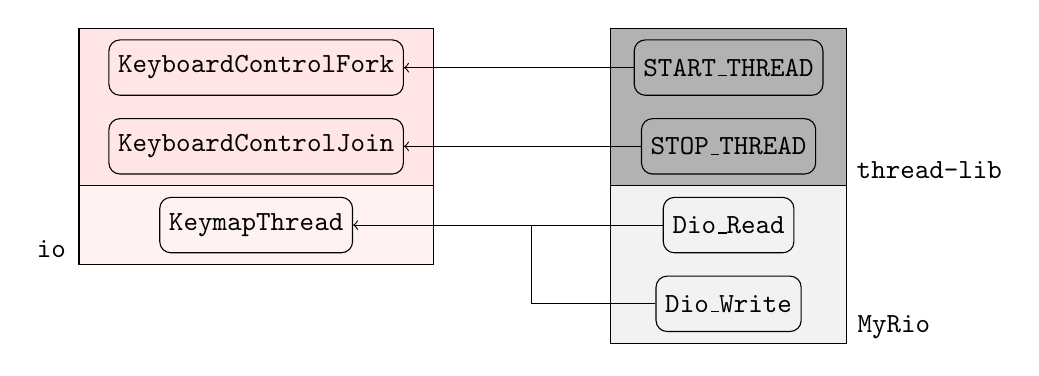
\begin{tikzpicture}
        \node[rectangle, draw, minimum width=4.5cm, minimum height=2cm, fill=red!10] at (0, -0.5) {};
        \node at (-2.6, -2.3) {\texttt{io}};
        \node[terminator] at (0, 0) (KeyboardControlFork) {\texttt{KeyboardControlFork}};
        \node[terminator] at (0, -1) (KeyboardControlJoin) {\texttt{KeyboardControlJoin}};
        \node[rectangle, draw, minimum width=4.5cm, minimum height=1cm, fill=red!5] at (0, -2) {};
        \node[terminator] at (0, -2) (KeymapThread) {\texttt{KeymapThread}};

        \node[rectangle, draw, minimum width=3cm, minimum height=2cm, fill=black!30] at (6, -0.5) {};
        \node at (8.55, -1.3) {\texttt{thread-lib}};
        \node[terminator] at (6, -0) (START_THREAD) {\texttt{START\_THREAD}};
        \node[terminator] at (6, -1) (STOP_THREAD) {\texttt{STOP\_THREAD}};

        \node[rectangle, draw, minimum width=3cm, minimum height=2cm, fill=gray!10] at (6, -2.5) {};
        \node at (8.1, -3.3) {\texttt{MyRio}};
        \node[terminator] at (6, -2) (Dio_Read) {\texttt{Dio\_Read}};
        \node[terminator] at (6, -3) (Dio_Write) {\texttt{Dio\_Write}};

        \draw[->] (START_THREAD) -- (KeyboardControlFork);
        \draw[->] (STOP_THREAD) -- (KeyboardControlJoin);
        \draw[->] (Dio_Read) -- (KeymapThread);
        \draw[-] (Dio_Write) -| (3.5, -2);
    \end{tikzpicture}
    \label{io-mdd2}
    \caption{\texttt{io} Keyboard Control Framework}
\end{figure}

This framework must be activated before Anti-Sway runs (via \texttt{KeyboardControlFork()}), otherwise it causes undefined behavior. Essentially, the threading function \texttt{KeymapThread()} continuously calculates which buttons, 1 through 9, are currently being pressed, and stores the result of that into a static variable (static to \texttt{io}), which is a boolean array of length 9 aliased as \texttt{Keymap} for convienence. Since all threads of this software belong to the same memory space, \texttt{GetReferenceVelocityCommand()} accesses this \texttt{Keymap} to determine which keys are pressed, and ultimately what velocity control signal to send.

This immediately should raise a red flag, because the keyboard resource is being shared amongst multiple threads. Thus, to solve this issue, a mutual exclusion lock is defined to represent the keyboard, and so \texttt{KeymapThread()}, \texttt{PressedDelete()}, and \texttt{GetReferenceVelocityCommand()} all have to use it to manipulate the keyboard's digital channels or the \texttt{Keymap}.

\begin{tcolorbox}[colframe=yellow!50!orange!50!black!75, title=Interesting Feature]
    A secret override of the MyRio function \texttt{char getkey()} is actually implemented in the \texttt{io} module, for the sole purpose of making it thread safe. It also uses the same lock that the above 3 functions use.
\end{tcolorbox}

\newpage

\subsection{Discrete Control: \texttt{discrete-lib}}

To accurately execute control laws, one must:
\begin{enumerate}
    \item Generate the Control Law
    \item Convert it to Discrete Format
    \item Execute it every BTI
\end{enumerate}
The second part of this becomes problematic because of the variability of controlling schemes. Our group in particular only requires relatively simple control schemes, while general control schemes require the use of Biquads to execute some control law, which can be confusing and uninterpretable within code. Thus, our group defines data types that help one program a control law simply by reading a control law diagram. We first start this explanation by the below dependency diagram:

\begin{figure}[H]
    \centering
    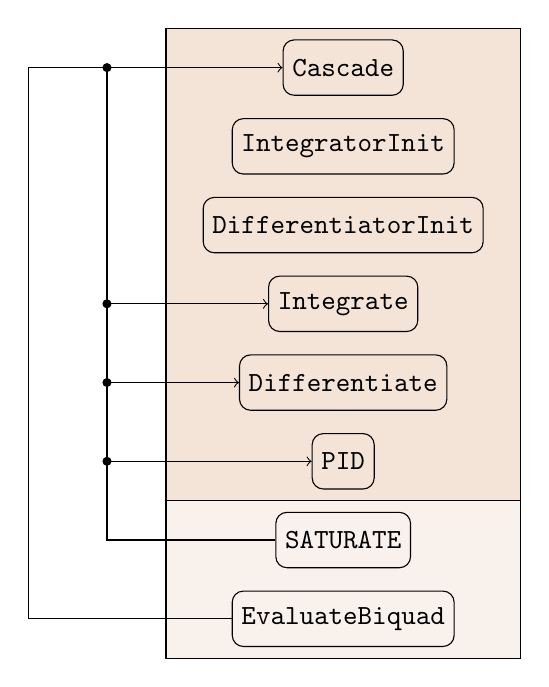
\begin{tikzpicture}
        \node[rectangle, draw, minimum width=4.5cm, minimum height=6cm, fill=red!10!brown!20] at (0, -2.5) {};
        \node[terminator] at (0, 0) (Cascade) {\texttt{Cascade}};
        \node[terminator] at (0, -1) (IntegratorInit) {\texttt{IntegratorInit}};
        \node[terminator] at (0, -2) (DifferentiatorInit) {\texttt{DifferentiatorInit}};
        \node[terminator] at (0, -3) (Integrate) {\texttt{Integrate}};
        \node[terminator] at (0, -4) (Differentiate) {\texttt{Differentiate}};
        \node[terminator] at (0, -5) (PID) {\texttt{PID}};
        \node[rectangle, draw, minimum width=4.5cm, minimum height=2cm, fill=red!5!brown!10] at (0, -6.5) {};
        \node[terminator] at (0, -6) (SATURATE) {\texttt{SATURATE}};
        \node[terminator] at (0, -7) (EvaluateBiquad) {\texttt{EvaluateBiquad}};

        \draw[->] (EvaluateBiquad) -- ++(-4, 0) |- (Cascade);
        \draw[-] (SATURATE) -- ++(-3, 0) -- (-3, 0);
        \draw[->] (PID)++(-3, 0) -- (PID);
        \draw[->] (Integrate)++(-3, 0) -- (Integrate);
        \draw[->] (Differentiate)++(-3, 0) -- (Differentiate);

        \filldraw[color=black] (Cascade)++(-3, 0) circle (0.05);
        \filldraw[color=black] (Integrate)++(-3, 0) circle (0.05);
        \filldraw[color=black] (Differentiate)++(-3, 0) circle (0.05);
        \filldraw[color=black] (PID)++(-3, 0) circle (0.05);
    \end{tikzpicture}
    \label{discrete-mdd}
\end{figure}

You can see this module is self-sufficient. This makes much sense as a library. The sole purpose of this library is to help easily implement control laws (the non-plant portion typically). Here are the functions:
\begin{itemize}
    \item \texttt{inline double Cascade(double input,
    Biquad sys[],
    int size,
    double lower\_lim,
    double upper\_lim)}: Applies a discrete transfer function, as a series of Biquads (bi-quadratics), to an input, with saturation limits.
    \item \texttt{void Integrator/DifferentiatorInit(Proportional gain,
    double timestep,
    Integrator/Differentiator *result)}: Initializes an \texttt{Integrator}, or \texttt{Differentiator}.
    \item \texttt{inline double Integrate/Differentiate(double input,
    Integrator *term,
    double lower\_lim,
    double upper\_lim)}: Integrates/Differentiates a signal, with saturation limits.
    \item \texttt{double PID(double input,
    Proportional *p,
    Integrator *i,
    Differentiator *d,
    double lower\_lim,
    double upper\_lim)}: Performs PID compensation on an input, with saturation limits. You can drop any of the PID terms by specifying NULL.
    \item \texttt{SATURATE(value, lo, hi)}: A macro that saturates value using the low (\texttt{lo}) and high values (\texttt{hi}).
\end{itemize}

Essentially, we have 4 control blocks, which is a general transfer function \texttt{Biquad}, an \texttt{Integrator}, \texttt{Differentiator}, as well as a \texttt{Proportional} (which is just an alias for a floating-point type). These compartmentalize control blocks in Control Law diagrams, and with the functions provided, allow us to write down a control law in code with relative ease. We will now dive more into these control blocks.

\subsubsection{Control Blocks: Control Made Easy}
There are some data structures to be aware of here though:
\begin{multicols}{3}
    \begin{center}
        \begin{lstlisting}[language=C]
typedef struct {
    double numerator[3];
    double denominator[3];
    double prev_input[2];
    double prev_output[2];
} Biquad;
        \end{lstlisting}
    \end{center}
    \columnbreak
    \begin{center}
        \begin{lstlisting}[language=C]
typedef struct {
    Proportional gain;
    double prev_input;
    double prev_output;
} Integrator;
        \end{lstlisting}
    \end{center}
    \columnbreak
    \begin{center}
    \begin{lstlisting}[language=C]
typedef struct {
    Proportional gain;
    double prev_input;
    double prev_output;
} Differentiator;    
    \end{lstlisting}
    \end{center}
\end{multicols}

Biquad, or biquadratic, is simply a transfer function as a ratio of 2 2nd order polynomials with respect to the delay operator ($z^{-1}$). Its first two fields and the integrator/differentiator's first fields indicate the form of each transfer function. The last two fields of all are essential to making sure each data type run properly. They originate from transforming their continuous counterparts via Tustin's transform:
$$\boxed{s = \frac{2}{T}\frac{1-z^{-1}}{1+z^{-1}}}$$

Thus, a discrete integrator or differentiator is defined by:
$$\boxed{K_ds = \frac{2K_d}{T}\frac{1-z^{-1}}{1+z^{-1}}}$$
$$\boxed{\frac{K_i}{s} = \frac{T}{2K_d}\frac{1+z^{-1}}{1-z^{-1}}}$$
And it is these coefficients on the right hand side that the gain is set to in both \texttt{Integrator} and \texttt{Differentiator}. A \texttt{Biquad} must be set by basically plugging in the Tustin Transform into the original continuous transfer function, and placing it into standard discrete form.

\begin{tcolorbox}[colback=yellow!10, colframe=green!20!black!70, title=C-Style Usage]
    You will notice these data types look like Objects. This is not a coincidence, as they are designed to behave as such. If this were C++, we could take this to a whole other level, not only by designating them as objects, but by leveraging operator overloading to make control law design more readable within code. For instance, the feedback path in the following Control Law:

    \begin{figure}[H]
        \centering
        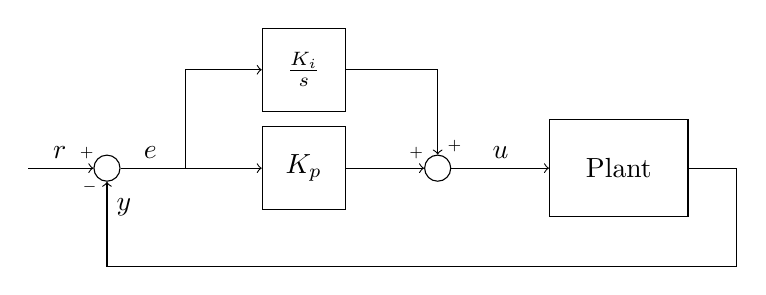
\begin{tikzpicture}
            \node[sum, name=feedback_sum] {};
            \node[block, name=int] at (2.5, 1.25) {$\frac{K_i}{s}$};
            \node[block, name=prop] at (2.5, 0) {$K_p$};
            \node[sum, name=pid] at (4.2, 0) {};
    
            \node[block, minimum width=5em, minimum height=3.5em, name=plant] at (6.5, 0) {Plant};
    
            \draw[->] (-1, 0) -- node [above, pos=0.9] {\tiny $+$} (feedback_sum);
            \draw[->] (feedback_sum) -- (prop);
            \draw[->] (1, 0) |- (int);
            \draw[->] (prop) -- node [above, pos=0.9] {\tiny $+$} (pid);
            \draw[->] (int) -| node [right, pos=0.95] {\tiny $+$} (pid);
            \draw[->] (pid) -- (plant);
            \draw[->] (plant) -| (8, -1.25) -| node [left, pos=0.97] {\tiny $-$} (feedback_sum);
    
            \node[above] at (-0.6, 0) {$r$};
            \node[right] at (0, -0.5) {$y$};
            \node[above] at (0.55, 0) {$e$};
            \node[above] at (5, 0) {$u$};
        \end{tikzpicture}
    \end{figure}

    as done with our code in C has to look like:

    \begin{lstlisting}[language=C]
        % // Ki and BTI_S is some defined constant
        Integrator i;
        Proportional p;
        IntegratorInit(Ki, BTI_S, &i);

        % // e is some floating-point type, presumably a double
        double u = p * e + Integrate(e, &i, POS_INF, NEG_INF);
    \end{lstlisting}

    but in C++, it could look like:
    \begin{lstlisting}[language=C++]
        Proportional p;
        % // Constructor is now direct
        Integrator i(Ki, BTI_S);

        % // Using `double operator*(ControlBlock b, double signal)' &
        % // `ControlBlock operator+(ControlBlock a, ControlBlock b)'
        double u = (p + i) * e;
    \end{lstlisting}
    which is much less verbose and matches the control scheme visually.

\end{tcolorbox}

However, these blocks alone do not solve everything. With general filters, it becomes difficult to actually make some convenient way to create any control block. You'd have to resort to making an algorithm that can factor any transfer function into a ratio of product series of 2nd order terms, and put that into an array of biquads, which is beyond the scope of this project

\newpage

\subsection{Modes: \texttt{idle}/\texttt{tracking}/\texttt{anti-sway}}

Now, we get to the section where we get to talk about how each of the modes are implemented. Since they all use the Fork-Join Framework, and the fact that they are all modes, they will look the same, so we use the same diagram to show how they work.

\begin{figure}[H]
    \centering
    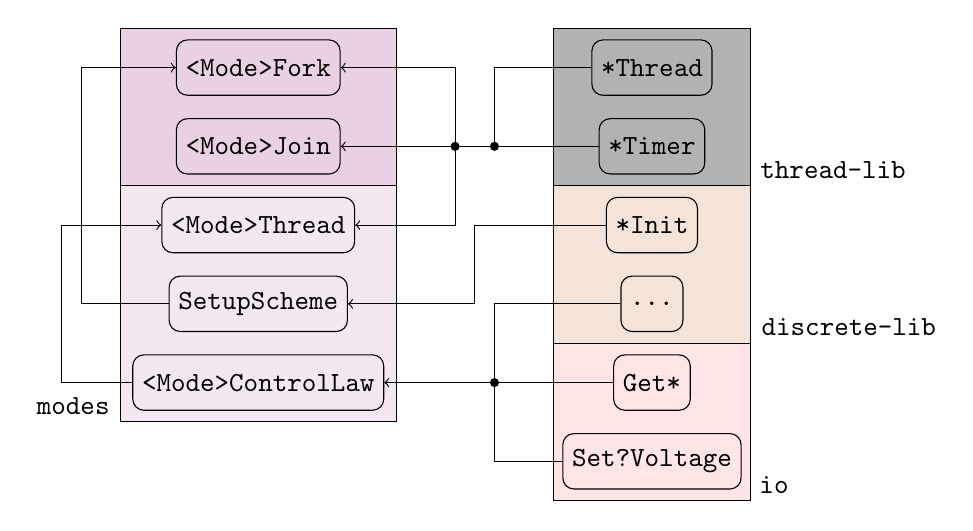
\begin{tikzpicture}
        \node[rectangle, draw, minimum width=3.5cm, minimum height=2cm, fill=blue!20!orange!20!violet!20] at (0, -0.5) {};
        \node[rectangle, draw, minimum width=3.5cm, minimum height=3cm, fill=blue!10!orange!10!violet!10]
        at (0, -3) {};
        \node at (-2.35, -4.3) {\texttt{modes}};
        \node[terminator] at (0, 0) (ModeFork) {\texttt{<Mode>Fork}};
        \node[terminator] at (0, -1) (ModeJoin) {\texttt{<Mode>Join}};
        \node[terminator] at (0, -2) (ModeThread) {\texttt{<Mode>Thread}};
        \node[terminator] at (0, -3) (SetupScheme) {\texttt{SetupScheme}};
        \node[terminator] at (0, -4) (ModeControlLaw) {\texttt{<Mode>ControlLaw}};

        \node[rectangle, draw, minimum width=2.5cm, minimum height=2cm, fill=black!30] at (5, -0.5) {};
        \node at (7.3, -1.3) {\texttt{thread-lib}};
        \node[terminator] at (5, 0) (Thread) {\texttt{*Thread}};
        \node[terminator] at (5, -1) (Timer) {\texttt{*Timer}};

        \node[rectangle, draw, minimum width=2.5cm, minimum height=2cm, fill=red!10!brown!20] at (5, -2.5) {};
        \node at (7.5, -3.3) {\texttt{discrete-lib}};
        \node[terminator] at (5, -2) (Init) {\texttt{*Init}};
        \node[terminator] at (5, -3) (Others) {\texttt{...}};

        \node[rectangle, draw, minimum width=2.5cm, minimum height=2cm, fill=red!10] at (5, -4.5) {};
        \node at (6.55, -5.3) {\texttt{io}};
        \node[terminator] at (5, -4) (Get) {\texttt{Get*}};
        \node[terminator] at (5, -5) (Set) {\texttt{Set?Voltage}};

        \draw[-] (Thread) -| (3, -1);
        \draw[-] (Timer) -| (3, -1);
        \draw[->] (3, -1) -- (ModeJoin);
        \draw[->] (2.5, -1) |- (ModeFork);
        \draw[->] (2.5, -1) |- (ModeThread);

        \draw[->] (Init) -- (2.75, -2) |- (SetupScheme);
        \draw[->] (Others) -- ++(-2, 0) |- (ModeControlLaw);
        
        \draw[->] (ModeControlLaw) -- +(-2.5, 0) |- (ModeThread);
        \draw[->] (SetupScheme) -- +(-2.25, 0) |- (ModeFork);

        \draw[-] (Get) -- ++(-2.5, 0);
        \draw[-] (Set) -| (3, -4);

        \filldraw[color=black] (3, -1) circle (0.05);
        \filldraw[color=black] (2.5, -1) circle (0.05);
        \filldraw[color=black] (3, -4) circle (0.05);
    \end{tikzpicture}
    \label{modes-mdd}
    \caption{\texttt{idle}, \texttt{anti-sway}, and \texttt{tracking} Module Dependency Diagram}
\end{figure}

You'll see that this is just the Fork-Join Framework, with the use of some additional functions. In this case, the function \texttt{<Mode>Thread} serves as the Thread Function, and is \texttt{static} because the user needs no access to it. For some clarity, the \texttt{...} within the \texttt{discrete-lib} module is any of the time-stepping functions for Control Blocks (so functions that time step a transfer function). The other two \texttt{static} methods in \texttt{modes} will be discussed in the next subsection, but they essentially assist with running the Control Laws. Idle Mode of course has no need for these functions because it is not running any control law.

\subsubsection{Multiaxis Control}

Because both Tracking and Anti-Sway Mode operate along 2 axis, there needs to be an efficient way to run both axes at the same time. Thus, each of these modules define a \texttt{struct} that encapsulates their `schemes':
\begin{multicols}{2}
    \begin{center}
        \begin{lstlisting}[language=C]
typedef struct {
    // Outer-loop Constant
    Proportional combined_constants;
    // Artificial Damping
    Proportional damping;
} TrackingControlScheme;
        \end{lstlisting}   
    \end{center}
    \columnbreak
    \begin{center}
        \begin{lstlisting}[language=C]
typedef struct {
    // Outer feedback
    Proportional outer_feedback;
    // Inner PI Proportional Gain
    Proportional inner_prop;
    // Innner PI Integral Term
    Integrator inner_int;
} AntiSwayControlScheme;
        \end{lstlisting} 
    \end{center}
\end{multicols}

Looking carefully, these both contain all the Control Blocks necessary to replicate the feedback path of each of the controllers. In each of these files, there are always 2 of these defined, one for each axis. And so with these `schemes', we use the following functions to utilize them:
\begin{itemize}
    \item \texttt{void SetupScheme(..., <Mode>Scheme \&scheme)}: Sets up the feedback path for the controller portion of the Control Law, which can involve the \texttt{DifferentiatorInit()} or \texttt{IntegratorInit()} functions.
    \item \texttt{void <Mode>ControlLaw(..., <Mode>Scheme \&scheme, int (* SetVoltage)(Voltage voltage))}: Executes one iteration of the Control Law, using the \texttt{scheme} to send a voltage through the parameter \texttt{SetVoltage}. The control laws use the discrete time library to do this.
\end{itemize}
Thus, this \texttt{<Mode>Scheme} data structure helps us seperate the control laws, \texttt{<Mode>SetupScheme} helps us setup each of the data structures, while \texttt{<Mode>ControlLaw} executes them independently, by passing one of \texttt{SetXVoltage()} or \texttt{SetYVoltage()}.

\subsubsection{Sensor Assurance: Idle Mode}
The purpose of Idle Mode is to check whether the sensors are working properly and that they increment in the right direction (they follow the sign convention established). During the operation of Idle Mode, the following message, which is updated regularly, is displayed:
\begin{center}
    \begin{tabular}{c}
        \begin{lstlisting}
P: (X.XXX, X.XXX) m
V: (X.XXX, X.XXX) m/s
A: (X.XXX, X.XXX) deg
        \end{lstlisting}
    \end{tabular}
\end{center}
Thus, by providing a print-out of the sensor measurements, we can verify whether the system is working properly by moving it around.
\begin{tcolorbox}[colframe=blue!50!black!70,title=Future Modification]
    Idle Mode has a bug. The velocity output is incorrect, because the BTI of this mode is distorted due to the user of \texttt{printf\_lcd()}. This was not an important issue because the main purpose of idle mode is simply to see that the sensors were working properly. However, if one wishes to make this reading more accurate, then you would want to make the measurement of the velocity (or just all of the measurements) and the printing of the measurements parallel tasks, which would involve yet another Fork-Join threading activity.
\end{tcolorbox}

\subsection{Data Requisition: \texttt{record}}
This section is a wrapper around the \texttt{matlabfiles} module. It simply adapts the functionality of the module to our particular uses. In particular, we want the ability to:
\begin{itemize}
    \item Record one-valued data
    \item Record data every BTI
\end{itemize}
So, this module helps us achieve that. Here, we have:
\begin{figure}[H]
    \centering
    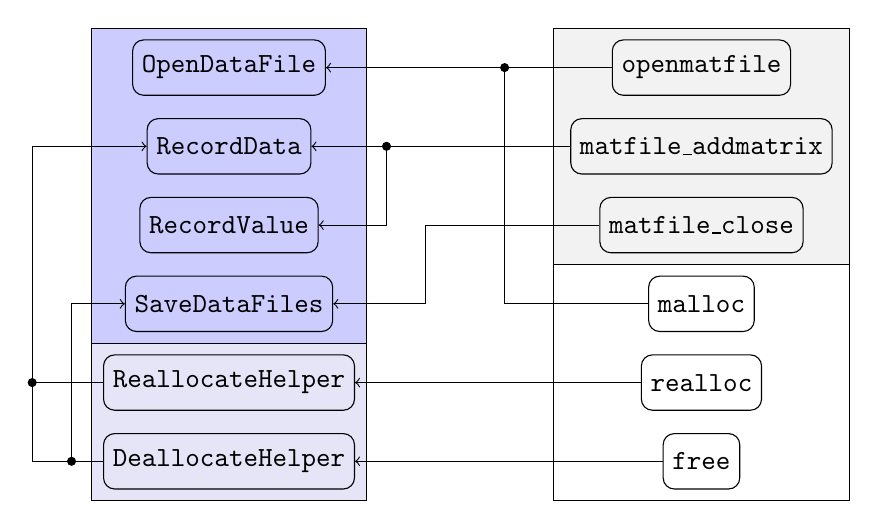
\begin{tikzpicture}
        \node[rectangle, draw, minimum width=3.5cm, minimum height=4cm, fill=blue!100!black!20!] at (0, -1.5) {};
        \node[terminator] at (0, 0) (OpenDataFile) {\texttt{OpenDataFile}};
        \node[terminator] at (0, -1) (RecordData) {\texttt{RecordData}};
        \node[terminator] at (0, -2) (RecordValue) {\texttt{RecordValue}};
        \node[terminator] at (0, -3) (SaveDataFiles) {\texttt{SaveDataFiles}};
        \node[rectangle, draw, minimum width=3.5cm, minimum height=2cm, fill=blue!70!black!10!] at (0, -4.5) {};
        \node[terminator] at (0, -4) (ReallocateHelper) {\texttt{ReallocateHelper}};
        \node[terminator] at (0, -5) (DeallocateHelper) {\texttt{DeallocateHelper}};

        \node[rectangle, draw, minimum width=3.75cm, minimum height=3cm, fill=gray!10] at (6, -1) {};
        \node[terminator] at (6, -0) (openmatfile) {\texttt{openmatfile}};
        \node[terminator] at (6, -1) (matfile_addmatrix) {\texttt{matfile\_addmatrix}};
        \node[terminator] at (6, -2) (matfile_close) {\texttt{matfile\_close}};
        \node[rectangle, draw, minimum width=3.75cm, minimum height=3cm] at (6, -4) {};
        \node[terminator] at (6, -3) (malloc) {\texttt{malloc}};
        \node[terminator] at (6, -4) (realloc) {\texttt{realloc}};
        \node[terminator] at (6, -5) (free) {\texttt{free}};

        \draw[->] (openmatfile) -- (OpenDataFile);
        \draw[->] (matfile_addmatrix) -- (RecordData);
        \draw[->] (matfile_addmatrix)++(-4, 0) |- (RecordValue);
        \draw[->] (matfile_close) -- ++(-3.5, 0) |- (SaveDataFiles);

        \draw[-] (malloc) -| (3.5, 0);
        \draw[->] (realloc) -- (ReallocateHelper);
        \draw[->] (free) -- (DeallocateHelper);
        
        
        \draw[->] (ReallocateHelper) -- ++(-2.5, 0) |- (RecordData);
        \draw[-] (DeallocateHelper) -| (-2.5, -4);
        \draw[->] (-2, -5) |- (SaveDataFiles);

        \filldraw[color=black] (3.5, 0) circle (0.05);
        \filldraw[color=black] (matfile_addmatrix)++(-4, 0) circle (0.05);
        \filldraw[color=black] (-2, -5) circle (0.05);
        \filldraw[color=black] (ReallocateHelper)++(-2.5, 0) circle (0.05);
    \end{tikzpicture}
    \label{record-mdd}
    \caption{\texttt{record} Module Dependency Diagram}
\end{figure}
The module works similarly to other file i/o modules, but with some special recording methods.
\begin{itemize}
    \item \texttt{FileID\_t OpenDataFile(char *name, char **entry\_names, int num\_entries)}: Opens a Data File, with specific entries to be recorded every BTI. This module keeps track of this file while its open. Returns a non-negative numeber that signifies the file, or negative if the operation failed.
    \item \texttt{int RecordData(FileID\_t file, double data[], int data\_length)}: Records the data into the entries specified from the above function into the given file. The field \texttt{data\_length} must be equal to \texttt{num\_entries} from the call to \texttt{OpenDataFile()} that was used to produce \texttt{file}. It is also expected that \texttt{data[i]} be data under the entry name \texttt{entry\_names[i]}, also from the call to \texttt{OpenDataFile()}. Returns 0 upon success.
    \item \texttt{int RecordValue(FileID\_t file, char *value\_name, double value)}: Records a singular data with a particular name into the data file.
    \item \texttt{int SaveDataFiles()}: Saves all data files and closes them. Returns 0 upon success.
\end{itemize}

Basically, \texttt{OpenDataFile()} is used to open a data file, with the names of every entry to be recorded per BTI. All this data will be saved as a big array. Then, during each of the modes, during a BTI, the data is sent to the file for 1 BTI using \texttt{RecordData()}. Then, to save all this into the file, at the end of the software, \texttt{SaveDataFiles()} is called during \texttt{Shutdown()} within the \texttt{setup} module.

\begin{tcolorbox}[colframe=yellow!50!orange!50!black!75, title=Interesting Feature]
    You will notice that this module is omitted from all the Module Dependency Diagrams. That's because it is unnecessary to the operation of the program, and thus is unnecessary when modifying the core behavior of the program. Even if placed in a Module Dependency Diagram, all it tells you is that data is being recorded.
\end{tcolorbox}

\subsubsection{Internal File Management: Data Buffers}
You may be wondering though what all the references to dynamic memory allocation/deallocation are for. Although this module is a wrapper for \texttt{matlabfiles}, it operates with a bit more independence. For starters, you will notice that the external representation of a file is this aliased integer, \texttt{FileID\_t}. However, the internal representation of this is the following \texttt{struct}:
\begin{center}
    \begin{tabular}{c}
    \begin{lstlisting}[language=C]
typedef struct {
    MATFILE *file;
    int num_entries;
    char **entry_names;
    int num_vals;
    int vals_capacity;
    double **entry_values;
} DataFile_t;
    \end{lstlisting}
    \end{tabular}
\end{center}

This data structure can be broken down into 3 portions:
\begin{enumerate}
    \item The first field is the actual representation of the file, which would be a \texttt{.mat} file.
    \item The 2\textsuperscript{nd} and 3\textsuperscript{rd} fields refer to the names of the arrays that will be recorded in this data file (and how many names there are). Recall this corresponds to the data we want to record every BTI for a particular mode.
    \item The last 3 fields refer to the actual data that the user has recorded. \texttt{num\_vals} and \texttt{vals\_capacity} refer to the number of values in each of the arrays the user has already recorded, and the capacity of the array that stores them, respectively. This of course implies that all entries have the same amount of data. Then, the last field is essentially an array of arrays.
\end{enumerate}

For the last field, the locations of the double arrays, as well as the double arrays themselves must be dynamically allocated to allow for flexibility, which is why we utilize dynamic memory allocation. You can view the last field as a 2D array\footnote{In fact, since pointers are usually viewed as an array, a double pointer is normally viewed as a double array, and that is so in this case - You could actually use double array syntax to access particular values within \texttt{entry\_values}}. Here's how this field is used:
\begin{enumerate}
    \item To start, each of the arrays within this 2D array is initialized with a set length during \texttt{OpenDataFile()}.
    \item Then, when \texttt{RecordData()} is called, the parameter \texttt{data} is copied into their corresponding locations within \texttt{entry\_values}, utilizing \texttt{num\_vals} to place them in the right spot for each array. However, when each of the arrays within \texttt{entry\_values} is full, the arrays are resized within \texttt{ReallocateHelper()} (via \texttt{realloc()}). 
    \item Finally, when \texttt{SaveDataFiles()} is called when the user turns off the software, this data is actually written into a \texttt{.mat} file.
\end{enumerate}

However, this module must handle doing this with multiple files at once, so how does it do that? Essentially, an internal variable is declared, which is an array of \texttt{DataFile\_t} structures, called \texttt{files}. The key here is \texttt{FileID\_t}. It aliases an integer, and it just so happens that that integer is the same as the index of the file location in \texttt{files}. Thus, you can use the \texttt{file} filed passed into \texttt{RecordData()} or \texttt{RecordValue()} to access the corresponding \texttt{DataFile\_t} by doing the operation:

\begin{center}
    \begin{tabular}{c}
        \begin{lstlisting}[language=C]
DataFile_t *f = files + file;
        \end{lstlisting}
    \end{tabular}
\end{center}

\newpage

\subsection{Error Handling: \texttt{error}}
This last module is not much of a module itself, but is important because its influence spans multiple modules. It defines:
\begin{itemize}
    \item The universal error variable, \texttt{u\_error}.
    \item Error codes that correspond to what error has occured if \texttt{u\_error != 0}.
    \begin{itemize}
        \item \texttt{ENKWN}: Unknown Exception
        \item \texttt{EOTBD}: Out of Bounds Error (Positional Limit)
        \item \texttt{EVTYE}: Velocity Bound Exceeded
        \item \texttt{ESTRN}: Angle Sensor Saturation Error
        \item \texttt{EENCR}: Encoder Error
    \end{itemize}
\end{itemize}

\subsubsection{Error State}
In the module \texttt{system}, there is the error state. During the operation of any of the Modes (\texttt{idle}, \texttt{tracking}, or \texttt{anti-sway}), if a universal error occurs (that is, \texttt{u\_error != 0}), the Error state triggers, and suspends the operation of the module. Some errors are unrecoverable (\texttt{ENKWN} currently is the only one). Other errors can be recovered by manually adjusting the system (\texttt{EOTB}, \texttt{EVTYE}, and \texttt{ESTRN}) are all examples of this, as you can place the system back within limits.

To be more precise about things, \texttt{EOTBD} and \texttt{EVTYE} can be triggered whenever trolley position or velocity is meausred via \texttt{GetTrolleyPosition/Velocity()} from the \texttt{io} module. \texttt{ESTRN} can be triggered whenever \texttt{GetAngle()} is called, also from the \texttt{io} module.

Going back to the Error State, the Error State will first inform the user of what error has occured. Then, if the error is recoverable, then the program will prompt the user to either reenter the program (via the MENU state), or to just exit. An example is shown below:
\begin{lstlisting}
    Error: An encoder(s) has failed..
    Press:
    1) Continue
    2) Exit
\end{lstlisting}
If an error is non-recoverable, then the message will simply inform about the error and stop the software.

\subsubsection{Static Error Codes v. \texttt{errno}}
You may be questioning not using \texttt{errno} or some style of it. \texttt{errno} for reference is the C version of a universal error code. However, \texttt{errno} is different for different threads, and so to achieve so, \texttt{errno} is not a variable, it is a macro that expands to a thread-local error variable. In our case, we want a universal error in the fact that it is shared by the entire program, which includes all threads.

\newpage

\subsection{Special Feature: Anti-Sway Mode Tuning}
\begin{tcolorbox}[colframe=red!75!black,colback=yellow!5, title=WARNING]
    This feature can potentially compromise user safety. Exercise caution when using this mode.
\end{tcolorbox}
Anti-Sway mode comes with a Tuning feature that allows it to optimize its controller parameters, particularly its inner-loop PI parameters. To turn this mode on, locate the commented line of code:
\begin{center}
    \begin{tabular}{c}
        \begin{lstlisting}[language=C]
            #define TUNING
        \end{lstlisting}
    \end{tabular}
\end{center}

and uncomment it. This will activate Tuning Mode. It is important to note that during Tuning mode, a reference velocity of $$\vec{v}=<0.15, 0.15> m/s$$ will automatically be applied for a set amount of time (2.75 seconds to be precise). During this time, it gathers data on the performance of the system, and uses this to update the PI parameters accordingly. Running this repeatedly will generate better and better system performance, and when you are satisfied with the performance, obtain the PI parameter values that Anti-Sway last produced, comment the above line of code, and set the parameter values within the code.

\subsubsection{Autotuning: Simplisitic Machine Learning Control}
We will now explain how exactly this method works. Consider the following PID controller:
\begin{figure}[H]
    \centering
    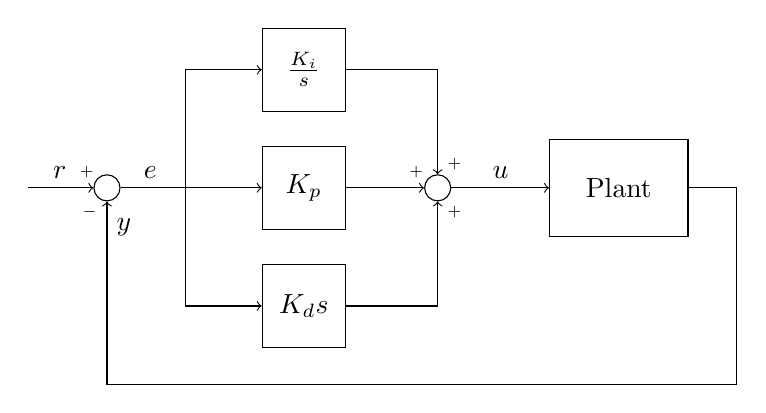
\begin{tikzpicture}
        \node[sum, name=feedback_sum] {};
        \node[block, name=int] at (2.5, 1.5) {$\frac{K_i}{s}$};
        \node[block, name=prop] at (2.5, 0) {$K_p$};
        \node[block, name=diff] at (2.5, -1.5) {$K_ds$};
        \node[sum, name=pid] at (4.2, 0) {};

        \node[block, minimum width=5em, minimum height=3.5em, name=plant] at (6.5, 0) {Plant};

        \draw[->] (-1, 0) -- node [above, pos=0.9] {\tiny $+$} (feedback_sum);
        \draw[->] (feedback_sum) -- (prop);
        \draw[->] (1, 0) |- (int);
        \draw[->] (1, 0) |- (diff);
        \draw[->] (prop) -- node [above, pos=0.9] {\tiny $+$} (pid);
        \draw[->] (int) -| node [right, pos=0.95] {\tiny $+$} (pid);
        \draw[->] (diff) -| node [right, pos=0.95] {\tiny $+$} (pid);
        \draw[->] (pid) -- (plant);
        \draw[->] (plant) -| (8, -2.5) -| node [left, pos=0.97] {\tiny $-$} (feedback_sum);

        \node[above] at (-0.6, 0) {$r$};
        \node[right] at (0, -0.5) {$y$};
        \node[above] at (0.55, 0) {$e$};
        \node[above] at (5, 0) {$u$};
    \end{tikzpicture}
    \caption{Generic PID Controller}
    \label{generic-pid}
\end{figure}

To train the above PID Controller, one must:
\begin{enumerate}
    \item Define the Loss Function. This Function defines what it means to ``lose'' performance. The greater the value of this function, the worse the controller performs. In this case, we optimize for reference tracking, in which case the loss function depends on the error signal $e$. Thus, our loss $$\mathbb{L}$$ becomes:
    $$\mathbb{L}(\bold{r}, \bold{y})=||\bold{r}-\bold{y}||_2^2=\sum_{t=0}^{T}{\left(r(t)-y(t)\right)^2}$$
    $$\mathbb{L}(\bold{e})=||\bold{e}||_2^2=\sum_{t=0}^{T}{e(t)^2}$$
    We square this because negative loss is bad. However, it is typically used for historical reasons (namely because working with square loss is normally what people do).
    \item Then, we calculate this loss. After running Anti-Sway Mode on Tuning Mode, we gather very controlled data about the performance of the system. Calculating the Loss allows us to measure the system performance and calculate what to do next.
    \item Now, we take the gradient of the loss that we just calculated, with respect to the PID parameters. This is often refered to as ``back-propogation'', and is an appropriate term here. We are training a State-Space System, which is a form of a Neural Network, and this particular term applies to this particular sort of system. Like a neural network, we use approximations to calculate this gradient. First we must gather the PID parameters as a vector:
    $$\bold{K}=
\begin{bmatrix}
    K_i \\
    K_p \\
    K_d
\end{bmatrix}$$
    Then, we can define the gradient as:
    $$\nabla_{\bold{K}}\mathbb{L}=\left(\nabla_{\bold{y}}\mathbb{L}\nabla_{\bold{u}}{y}+\nabla_{\bold{r}}{\mathbb{L}}\nabla_\bold{u}{\bold{r}}\right)\nabla_{\bold{K}}u$$
    $$\nabla_\bold{K}{\mathbb{L}}=\sum_{t=0}^{T}{\left(2e(t)\frac{\left(\frac{\partial r}{\partial y}-1\right)\frac{\partial y}{\partial u}+\left(1-\frac{\partial y}{\partial r}\right)\frac{\partial r}{\partial u}}{1-K_p\left(\left(\frac{\partial r}{\partial y}-1\right)\frac{\partial y}{\partial u}+\left(1-\frac{\partial y}{\partial r}\right)\frac{\partial r}{\partial u}\right)}
    \begin{bmatrix}
        \int{e(t)d\tau}+\frac{\partial}{\partial K_i}\left(K_d\frac{\partial e}{\partial t}+K_i\int{ed\tau}\right) \\
        e(t)+\frac{\partial}{\partial K_p}\left(K_d\frac{\partial e}{\partial t}+K_i\int{ed\tau}\right) \\
        \frac{\partial e}{\partial t}+\frac{\partial}{\partial K_d}\left(K_d\frac{\partial e}{\partial t}+K_i\int{ed\tau}\right)
    \end{bmatrix}\right)}$$
    $$\nabla_\bold{K}{\mathbb{L}}=\sum_{t=0}^{T}{\left(2e(t)\left(\left(\frac{\partial e}{\partial u}\right)^{-1}-K_p\right)^{-1}
    \begin{bmatrix}
        \int{e(t)d\tau}+\frac{\partial}{\partial K_i}\left(K_d\frac{\partial e}{\partial t}+K_i\int{e(t)d\tau}\right) \\
        e(t)+\frac{\partial}{\partial K_p}\left(K_d\frac{\partial e}{\partial t}+K_i\int{e(t)d\tau}\right) \\
        \frac{\partial e}{\partial t}+\frac{\partial}{\partial K_d}\left(K_d\frac{\partial e}{\partial t}+K_i\int{e(t)d\tau}\right)
    \end{bmatrix}\right)}$$
    where all partial derivatives are approximated using a 1\textsuperscript{st} order backward Euler approximation. Each operand in the summation is reffered to as a unit gradient, because it is the contribution of a particular data point to the gradient. Notice that we take the derivative with respect to the reference signal in some partial derivatives. Unlike in most PID systems where the reference signal is mostly constant, the reference to the PI controller for Anti-Sway is not, so that must be accounted for.
    \item Finally, we update the PID parameters using the gradient:
    $$\bold{K}_{n+1} \leftarrow \bold{K}_{n} - \eta \nabla_{\bold{K}}{\mathbb{L}}$$
    \item We have completed what is called an Epoch of Gradient Descent. Essentially, we repeat until convergence, or until we want to.
\end{enumerate}

    Essentially this should be done over and over again until the loss stays roughly the same. One thing to note though, is that the nature of the partial derivatives with respect to the PI parameters demand that we carry out step 4 for only one parameter at a time for accuracy sake. If we were to step both at a time, we wouldn't really know the effect of changing particular parameters. Thus, what actually is executed is called Coordinate Descent. However, that is not possible, as physical noise prevents us from doing this (will discuss later). To see the result of this, please refer to the Capstone Final Paper.

\newpage

\section{Discussion}
\subsection{Encoder Issues}
If you inspec the code, you will notice that we did not use the universal error code for Encoder Failure (\texttt{EENCR}). This was initially used to detect encoder failures (for the issue mentioned in the Capstone Final Report), but was soon replaced by something else. This can be useful in detecting and triggering a universal error on continuous encoder failure, which is something that should be implemented.

In the future though, an ideal solution would be to simply fix the encoder, but even then, you would still want to have this error in the event that some future error renders a mechanical failure.
\subsection{Gradient Descent Issues}
This method was chosen to tune Anti-Sway because not all the innate system parameters can be easily deduced (particularly, friction and damping). Because we apply Gradient Descent to a Physical System and not a Simulated System, many issues emerge. The result of these issues however, is the early termination of this algorithm, and unfortunate as it is, technically yields us the best parameters. We will talk about the most apparent issues:
\subsubsection{Measurement Noise}
Although our sensors are very accurate, they will never measure values as idealy as a simulation does. Thus, some issues arise, and in particular, a very bad issue arises when two successive sensor, actuator, or sensor/actuator derived measurements end up the same. Take the following partial derivative, with variables defined in Figure \ref{generic-pid}:
$$\frac{\partial u}{\partial y}$$
In Figure \ref{generic-pid}, $y$ is a variable that would be measured by a sensor. If two successive measurements of $y$ are the same, that means that the partial derivative is infinite. This would be okay if the system were actually staying at the same $y$, but in a continuous system this is nearly impossible to find. If $y$ were constant, the most probably explanation is that the system has reached steady state, in which case the loss from that data point would be 0 and it doesn't affect Gradient Descent. But if $y$ were constant at a non-steady state point in time, that would adversely affect the gradient. Thus, in our algorithm, we throw away such unit gradients where the data point causes it to be ill-defined.

This brings up the question though of whether this is okay to do, because the very act of throwing points we don't like away could bias the gradient. There is a more scientific way to settle this particular question, but through much observation, it appears as this so-called ``failure'' of a unit gradient is random. If it is random, we can validly say that this is still a valid form of Gradient Descent, called ``Stochastic Gradient Descent'', in which we choose random point(s) to contribute to the gradient.

In our case though, different amounts of unit gradients fail through each Epoch of Gradient Descent, even though it stays random, which is to suggest that the probability of unit gradient failure happens at some $p$ and is i.d.d. (independent and identically distributed), but the value of $p$ changes between each run. Thus, consider our modified gradient $\nabla_K\mathbb{L}'$, which is a random variable because of this. The expectation of this gradient is the sum of the expectation of the unit gradients, which is 0 iff it fails and its true value iff it doesn't fail (a Bernoulli Random Variable). Thus:
$$\mathbb{E}[\nabla_K\mathbb{L}']=\sum_{t=0}^{T}{\mathbb{E}[\nabla_K\mathbb{L}(t=t)]}=\sum_{t=0}^{T}{p\nabla_K\mathbb{L}(t=t)}=p\sum_{t=0}^{T}{\nabla_K\mathbb{L}(t=t)}=p\nabla_K\mathbb{L}$$

which means that its expected to simply be a proportion of our real gradient. Thus the expectation of the update step during gradient descent is:
$$K_{n+1} \leftarrow K_{n}-\eta p \nabla_K\mathbb{L}$$
which is still valid, its now only that the learning rate effectively changes every iteration. This can be solved though by normalizing the gradient by the number of unit gradients that contribute to it, as in this model, $p$ is:
$$p \approx \frac{\#\ successful\ unit\ gradients}{\#\ total\ unit\ gradients}$$

\subsubsection{Physical Noise}
Physical noise is also in issue on many fronts. We want to see how the model does on the same set of conditions every Epoch, but that is impossible to assure since the initial conditions will change every time, as well as other factors.

However, what is more concerning is that at higher PI gains, the physical system starts experiencing what appears to be some resonance effect, which causes the trolley to physically shake, messing up the training regimen. However, what ends up happening is that the gradient actually directs the parameters to increase by an accelerating amount along the axis of shaking (the Y axis in our case). This could be an error in the code. However, this could also be due to a general issue with noise, which is that it constantly changes the loss hypersuface.

Essentially, what gradient descent does is that it follows the ``derivative'' of the loss function until it reaches a minimum in the ``Loss'' hypersurface (In our case, it is really just a 3 dimensional surface, but in the general PID case, it is a 4 dimensional surface, which is why it is refered to as a hypersurface). The primary issue with noise is that it changes the nature of the system and ultimately the model that we are trying to match with tuning, which changes this loss surface, and the magnitudes of our gradient descent algorithm.

A secondary effect though has to deal with the Loss Hypersurface's Convexity. Essentially a surface is convex iff every local minimum is the global maximum. Thus if we know the Loss Hypersurface is convex, we know that Gradient Descent will always go to the global minimum (which is what we want to achieve - the lowest possible loss). However, a non-convex surface has a global minimum, but also one or several local minima. Thus, if gradient descent is initialized a particular way, it can tend towards a local minima, which does not maximize the performance of our controller in the best way possible.

Essentially, using Gradient Descent on a PI or PID controller is generally a non-convex problem. However, the introduction of noise further frustrates the algorithm because noise can adversely affect the gradient in such a way that it changes the trajectory of Gradient Descent to fall into a less optimal loss.

\newpage

\section{Conclusion}

It is with confidence that we can state that this software has served our needs well, and its sound architecture has helps us save a lot of time, as well as make a better control system. It is also with confidence that we say if this project is to be continued, more improvements must be made to it so that it will be more robust. I hope this has been a good guide to the inner workings of the software. It is by no means perfect, but it should convey enough information about what is going on.

\newpage

\section{Appendix}
\subsection{Code Base}
Our code base is located within this GitHub: \hyperlink{https://github.com/me8927/Capstone-Stuff}{Anti-Sway Capstone GitHub}. You will find the following folders:
\begin{enumerate}
    \item \texttt{src}: The source code for the embedded software. Make sure you also have the entire \texttt{T1} library installed to run this.
    \item \texttt{Software Documentation}: The Latex Files for this document
    \item \texttt{Code Documentation}: The code-level documentation for this software. You can access \texttt{html}, which displays this in a website (download this folder and click on \texttt{annotated}), or \texttt{latex}, for which you can find latex files to view this documentation in pdf format (you will want to compile \texttt{refman.tex} within this folder).
    \item To access the website, simply visit \hyperlink{https://nguy8tri.github.io/Anti-Sway-Capstone/index.html}{Code-Level Documentation for Anti-Sway Capstone}
\end{enumerate}

\end{document}
